%\documentclass[a4paper,titlepage,12pt,DIV10,BCOR0.5cm,headinclude]{scrbook}
\documentclass[a4paper,titlepage,12pt,DIV10,BCOR0.5cm,headinclude]{article}
\DeclareFixedFont{\MyCode}{T1}{pcr}{m}{n}{10pt}
\usepackage[latin1]{inputenc}
\usepackage[T1]{fontenc}
\usepackage{eurosym}
\usepackage[pdftex]{graphicx}
\usepackage{ae}
%\usepackage{a4}	%for scrbook
\usepackage{lscape}
% \usepackage{url}
\newenvironment{mytinylisting}
{\begin{list}{}{\setlength{\leftmargin}{1em}}\item\tiny\bfseries}
{\end{list}}

\usepackage{listings}
\usepackage{setspace}
\lstset{numbers=none, numberstyle=\tiny, numbersep=2pt, basicstyle=\footnotesize}
\lstset{language=xml}

\pagestyle{plain}
\pagenumbering{arabic}


\begin{document}
\onehalfspacing
\parindent 0pt

\tableofcontents
\newpage
%**************************************************************************************
\section{Introduction}
%**************************************************************************************
\textit{Information processing systems have grown up around the globe at "Web speed", only slightly slower than "warp speed" in science fiction.} \cite{Luckham05}
\\\\
The backbone of IT systems used in todays life are based on distributed systems that are wired together by the global spanning Internet. The Internet has become the foundation of the twenty-first-centuries daily business and increased the volume of information passed beween enterprises and rose the demand for shorter decision-making cycles significantly. Based on this distributed computing architecture banks, insureance companies, governments, hospitals, military, airports and many more use these technologies as a result of growing needs to reduce costs, increase competitiveness and increase the time to market. Almost no enterprise can go around those technologies in daily life without a loss of competitiveness even if it is only the basic communication facility like the email service deployed.
\\\\
\textit{A distribute system is a collection of independent computers that appears to its users as a single coherent system.} [Tanenbaum1]
\\\\
The world has become a global market and the Internet is the highway connecting each other on the globe. On a virtual global trade market a bunch of enterprises are connected together so they can share resources or automate trading process to fullfill the needs for flexibility on a global market. E-Commerce processes became more and more complex and highly asynchronous. Enterprise systems supporting a wide range of enterprise collaborations including managment support tasks like supply chain managment (SCM), business intelligence (BI) in general or enterprise resource planning systems (ERP). The typical application in this infrastructure is to automate the workflows of commercial enterprises like transaction processing in the financial sector or the general support of electronic collaborations. As business process have grown out traditional synchronous workflow to support electronic collaborations, especially in B2B markets, more sophisitcated techniques have been developed to support them. E-business processes became complex, highly parallel and asynchronouse with far less human involment \cite{LuckhamManensPark}. 
\\\\
\textit{Today thousands of business-level events per second are being communicated across the IT layers of some enterprises. These numbers will increase with activity in the global eMarketplace.} [Luckham06]
\\\\
For example an auto manufacturer can automatically place orders around the globe for specific parts and receive delivery offers so that the production can be done in a "just in time" manner without the time consuming and error prone work of humans while he is reducing the inventory costs. Furthermore this way of doing business is fast and unchallengeable cheap. These collaboration may manifest in either a horizontal way or vertical way. The horizontal collaboration is restricted to a specific industry where business is centered around hubs. The vertical is opened to different clients that can purchase goods from a supplier. More typical applications are the well known Supply Chain Managment or Enterprise Resource Planning. Almost every deparment can benefit from these systems like marketing with CRM applications, the manangment by business intelligence informations and ERP systems, the sales and buying department using supply chain managment systems and so on. As you can see not every application must go out of the enterprises bounds.
\\\\
The main benefit of this so called "enterprise systems" are:
\begin{itemize}
	\item reduced costs
	\item lower inventory levels
	\item faster time to market
	\item increase profitability
	\item increate competitiveness
\end{itemize}
The main drawback of such systems is that they are "event driven" systems where billions of events on different granularity levels fly across our networks. The point is that there is no technology that helps us to look at those events in a human understandable way and the requirement of looking at these information in almost real-time has risen. Another point is that the event exchange is based on hetrogenouse systems where every enterprise has it's own implementation or even every department. As Luckham says:
\\\\
\textit{To be sure, given the primitive tools we have at the moment, we can see the events. But making sense of them is the problem!} [Luckham05]
\\\\
With currently available tools we can monitor the information running across on our networks and we can testify if a router for example is overloaded but we can't make statements about events or activities in a business level manner. What people really need are answears like:
\begin{itemize}
	\item "Why is it that most of the time one third of my shipment is damaged after delivery to London?" The answear would result in the analysis of the events generated by the logistic and accounting enterprise systems. So you could find by analyzing those event streams that most of the shipments went out with a specific carrier that is responsible for these endresults.
	\item "Is my delivery in time?". The system can detect the current location based on events from a tracking service like the one offered by UPS for instance.
	\item "Why has the customer rejected the delivery?". You would have to follow back all the process events back to the start to find the root of his problems.
	\item "What triggered my order?"
\end{itemize}
As you can see it would be quite difficult to answear these questions based only on event monitoring on a low level. The real pain would be to track back problems because you don't have a causal tracking of events. You just simply don't know what caused something to fire an event. The most logic approach would be to the root back is the temporal order of the events. No! That won't work out ... events can happen parallel and in a disordered way next to the most important problem that you have got just too many of them, a lot of the events are just not relevant by themselfes and their source is distributed across multiple system! Especially the last point is very important in e-commerce systems where different systems perform multiple actions to achieve something. It is vital for business to understand what happens on the process level to analyze the behaviour in order to be able to extract knowledge for decision making. As business in general has accelerate the according processes have to be adapted continuously to keep on with the challenge of a global competition. This development cries for new real-time event-based technologies.
\\\\
\textit{A key to understanding events is knowing what caused them - and haveing that causal knowledge at the time the events happen. The ability to track event causality is an essentail step toward managing communication} [Luckham05]
\\\\
This means that we need to find ways to look at "high level events" in order to be able to answear strategic and business problems or to create decisions based on these data. The traditional assumption was that you can make analysises and decision based upon a load of historic data collected but this has changed over time. Today we are facing a great demand by organizations requireing immediate access to information in a closed loop real-time manner. 
\\\\
The system developed in this diploma thesis provides an infrastructure to organize and manage events in way that a user can track down event causalities according to different standpoints. More on this topic later. First we need to understand what exactly an event is, where they come from, what makes them so important and how they fit into a common IT architecture.

%**************************************************************************************
\section{Events, Correlations and their sources}
%**************************************************************************************

%**************************************************************************************
\subsection{Enterprise systems}
%**************************************************************************************
Enterprise systems can be layered to get an abstract view to handle the complexity under the hood. As we mentioned before the characteristics of an enterprise systems are:
\begin{itemize}
	\item They are hetrogenouse systems.
	\item They are connected by a network (usually the Internet).
	\item The communication is event driven.
	\item Each system provides a service or performs a task.
\end{itemize}

According to [Tanenbaum1] this layered view is organized in this way:
\\\\
%**********************
\begin{figure}[!hbt]                               
	\centering                                           
	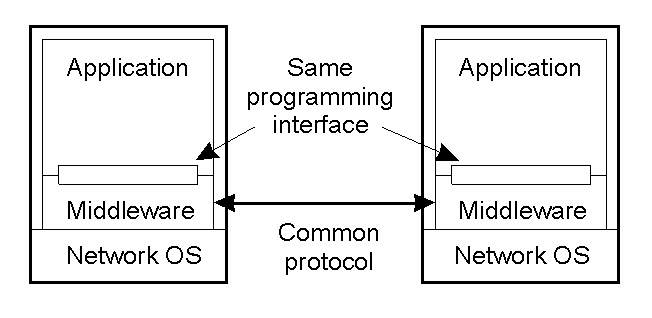
\includegraphics[width=1\textwidth]{pics/middlewareComm.jpg}
	\caption{Middleware based system [Tanenbaum1]}             
	\label{fig:MddlewareComm}
\end{figure}  
%**********************
%**********************
\begin{figure}[!hbt]                               
	\centering                                           
	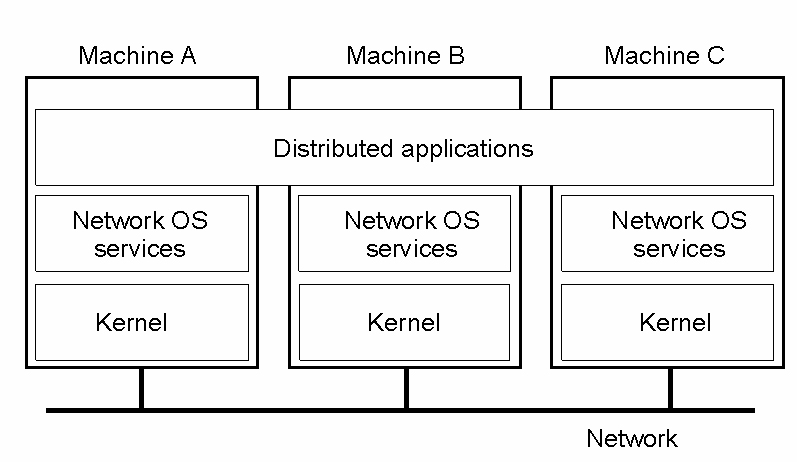
\includegraphics[width=1\textwidth]{pics/middlewareGeneral.jpg}
	\caption{Middleware based system [Tanenbaum1]}             
	\label{fig:MiddlewareGeneral}
\end{figure}  
%**********************
If you take a look from the top, from the users point of view he will get a homogenouse view of the system. Using the applications and developing them you won't have to take care about the underlying hetrogenity. It provides a single and coherent view to it's users. The rise of client/server application architectures where system components access remote infrastructure and functionality to accomplish their own tasks has led to the need to decouple communication parties to assure the need for scalability in the current IT infrastructures.
\\\\
To get a better understanding take the example from [Tanenbaum1]:
\\\\
Orders are placed from different types of clients like notebooks connected to the network, from the telephone network or cell phones. Those incoming orders are processed by a workflow system and the result is a new internal shipping order from the planning department and a billing order from the accounting. The users are not aware at all where those forwarded orders physically come from it appears that they are from a single central authority.
%**************************************************************************************
\subsection{Middleware Layer}
%**************************************************************************************
What makes this possible is the additional middleware layer that helps to hide the hetrogenity of the underlying platforms and improves transparency. The DOS is not intended to handle a collection of independent computers and a NOS doesn't provide a  view of a single coherent system. There are several models/paradigms describing the middleware layer:
\begin{itemize}
	\item Plan 9 was the first approach which treats everything as a file because that can be shared by several processes in the unix world and the communication is reduced to accessing files.
	\item Remote Procedure Calls (RPCs) allows to call functions and pass parameters on a remote machine. The callee doesn't know anything about the location of the remote function which can be on a machine physically somewhere else on the world.
	\item Distributed objects describes the method to invoke objects in a transparent way on remote machines by providing interfaceses of those objects.
	\item The message oriented paradigm takes care about providing the same communication facilities so that systems can talk to each other. The content of the information itself is ignored by these type of middleware models.
\end{itemize}
%**************************************************************************************
\subsection{Communication Paradigms}
%**************************************************************************************
There are different communication paradigms we have to be aware of before continuing:
\begin{itemize}
	\item \textbf{Transient communication} stores a message only as long as the sender and receiver is up and running.  
	\item \textbf{Persistent communication} on the other hand stores a message as long as the receiver retrieves it.
	\item \textbf{Asyncronouse communications} characteristic is that it sends a message and doesn't wait for a notification so it can keep on working without a halt.
	\item Applying \textbf{Syncronouse communication} will result in a delay for the sender until a received notification will come in from the receiver. 
	\item \textbf{Broadcast} means that a sender is communicating to multiple receivers.
	\item \textbf{Point to Point} communication is simply that one communication links has been established between sender and receiver.
\end{itemize}

Today the message oriented middleware paradigm has become one of the communication pillars of todays enterprise systems. It is the most common communication facility for exchanging information. There are different ways of organizing message oriented middlewares, but the most important is the message queing type. 
\\\\
\textit{Message-queing systems provide extensive support for persistent asynchronous commuication} [Tanenbaum1]
\\\\
In practice each application has got it's own message queue or several applications share one queue. This enables applications to communicate with eachother by inserting messages into specific queues using message-queing systems. This allows a loosely-coupled communication between systems. The inserted messages are pending in the queue as long as the receiver fetches it from the queue. So neither the sender or the receiver client has to be online if a message has been deployed in a queue. An important fact is that usually message-queueing systems don't gurantee the delivery of the sent messages. However there are mechanisms available in a variety of products to ensure the success of message transactions. This message based style communication bears the potential to integrate new autonomous, heterogeneous components into complex systems that are easy to evolve and scale \cite{LudgerFiege05}.
\\\\
As messages can contain any form of data the integration into a distributed system can lead to problems as applications provide different data formats. Message Brokers are an important application to act as a gateway between message-queuing systems. It transforms messages into a format that can be read by the different communication partners.
\\\\
The layering according to [Tannenbaum1] is a very simple point of view as he only wants to show how a middleware can enable a transparent and single coherent view of a system. David Luckham introduces a slightly deeper granularity of the high level overview of an distributed, event-driven system in order to be able to understand the importance of events for an enterprise.
\\\\
\textit{Layered IT systems present another dimension in the search for new ways to understand the events that happen in them.} [Luckham05]
%**********************
\begin{figure} [h]                        
	\centering                                           
	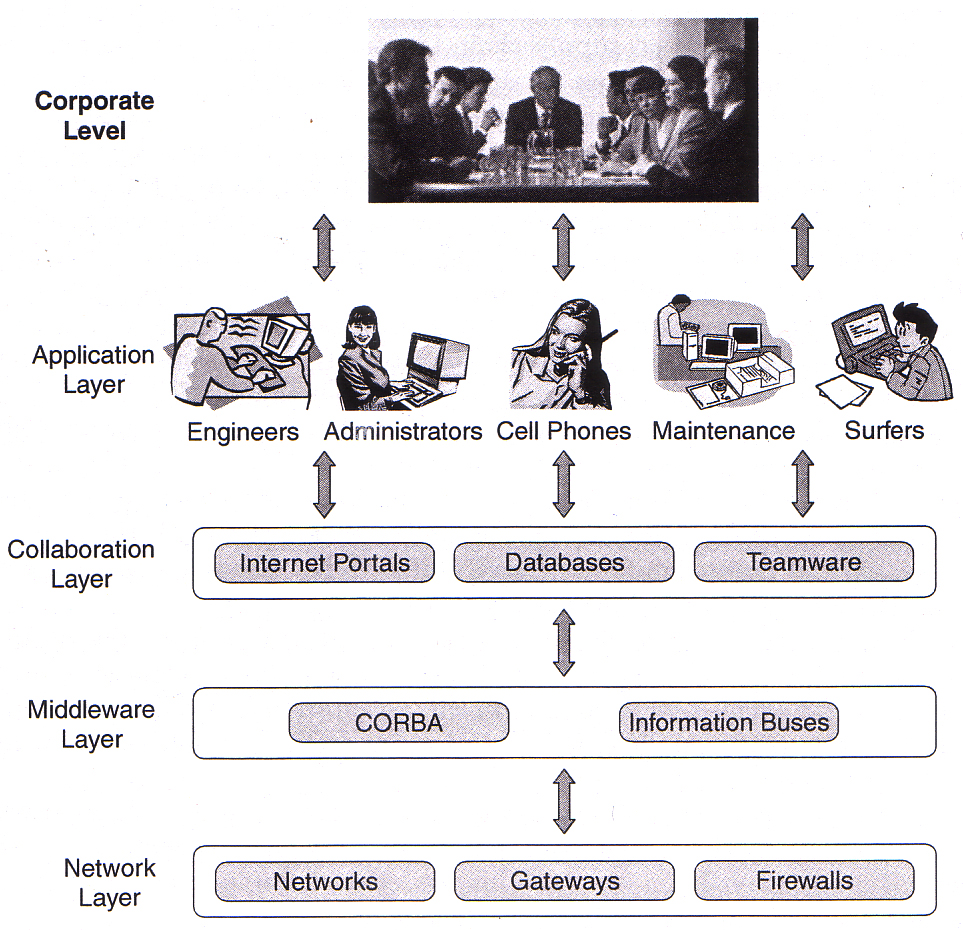
\includegraphics[width=1\textwidth]{pics/corporateLayer.jpg}
	\caption{Enterprise System Layering [Luckham05]}             
	\label{fig:EnterpriseSystemLayer}
\end{figure}  
%**********************
\begin{itemize}
	\item \textbf{Corporate Level:} At this layer enterprises plan and transact their business. Applications like accounting, inventory, spreadsheets, e-mail clients, calendars, webbrowsers and in general interfaces to other services belong in here.
	\item \textbf{Application Layer:} At this layer events are generated on a high level by the user where they signify activities like sending an e-mail. Actually many events generated at this layer are not simply one event rather they are aggregated to a high level event from the events generated by the layers underneath.
	\item \textbf{Collaboration Layer:}: This layer provides the the basic infrastructure for applications like databases, e-mail servers, web servers and so on. The line between the application layer and the collaboration layer can be blury.
	\item \textbf{Middleware Layer:} As mentioned above this is a very important part because it lets enterprise systems talk to each other.
	\item \textbf{Network Layer:} This layer is the basic layer where everything builds on top of it. At this layer only low level events are generated to transport information from A to B.
\end{itemize}

%**************************************************************************************
\subsection{On events}
%**************************************************************************************
As we talk quite a lot about passing messages back and forth in enterprise systems what meaning has an \textit{event} exactly? 
\\\\
In context of computer science an event is used to control the flow of a program. A well known application are user interfaces where triggered user interface elements generate events to start a processes.
\\\\
According to [Luckham05] an event is defined as:
\\\\
\textit{An event is an object that is a record of an activity in a system. The event signifies the activity. An event may be related to other events.}
\\\\
Ludger Fiege describes an event in his thesis as:
\\\\
\textit{Any happening of interest that can be observed from within a computer is considered an event}\cite{LudgerFiege05}
\\\\
For better understanding we follow \cite{Lamport78} and assume that we have a distributed system holding processes for receiving and sending messages. The dot represents occured events and the dotted line represents a message. The vertical direction represents the time and the horizontal the space dimension.
%**********************
\begin{figure}                         
	\centering                                           
	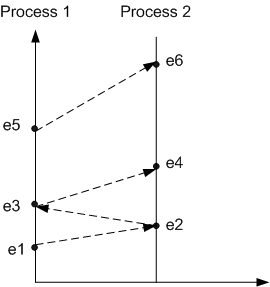
\includegraphics[width=0.6\textwidth]{pics/lamportEvent.jpg}
	\caption{Events and Messages}             
	\label{fig:LamportEvent}
\end{figure}  
%**********************
There are three aspects an event covers [Luckham05]:
\begin{itemize}
	\item \textit{\textbf{Form:} An event is an object containing attributes or data components.}
	\item \textit{\textbf{Significance:} An event signifies an activity}
	\item \textit{\textbf{Relativity:} An activity is related to other activities by time, causality and aggregation.}
\end{itemize}
Furthermore an event ussually contains an unqiue id and a timestamp to mark the creation of that event. 
\\\\
An example for events used in our system as a simulation model would be an OrderReceived event that signifies the activity of a posted order for some products:
\\\\
\begin{lstlisting}[caption=OrderReceivedEvent, label=lst:OrderReceivedEvent]{OrderReceivedEvent}
<OrderReceived>
	<OrderId>14765</OrderId>
	<DateTime>2005-10-31T11:31:02</DateTime>
	<DeliveryDate>2005-11-12T06:00:00</DeliveryDate>
	<Destination>Madrid</Destination>
	<ProductCollection>
		<Product>		
			<ProductId>Arzeutic</ProductId>
			<Amount>700</Amount>
		</Product>	
	</ProductCollection>
</OrderReceived>
\end{lstlisting}

Events are generated from different sources and different types. Normally they use some standard like the XML format. The received events must be transformed into higher level form in order to be able to work with them. This transformation is provided by adapter compontents.
%**************************************************************************************
\subsubsection{Relationsships}
%**************************************************************************************
According to [Luckham05] there are three important relationships between events:
\begin{itemize}
	\item \textbf{Time:} Relates events according to their temporal occurence
	\item \textbf{Cause:} Relates events according to their causal relationships. A causal relationship is given when an event a caused another event b in a direct or indirect way.
	\item \textbf{Aggregation:} Aggregates event to high level events based upon different criterias like time, causality or content patterns.
\end{itemize}
Following Luckhams [Luckham05] proposal that a timestamp defines the time relationship between events is not as easy as he says that you can determine by the time dimension that \textit{event A happened before event B}. Leslie Lamport adresses this problem \cite{Lamport78}:
\\\\
\textit{In a distributed system, it is sometimes impossible to say that one of two events occured first. The relationship "happened before" is therefore only a partial ordering of the events in the system.} \cite{Lamport78}
\\\\
The happens-before relation "$\rightarrow$" can be defined for following situations:
\begin{itemize}
	\item If a and b are events in the same process, and a comes before b, then a $\rightarrow$ b.
	\item If a is an event sending a message from one process and b is an event receiving the message from another process then a $\rightarrow$ b.
	\item The happens-before relation "$\rightarrow$" is transitive: a $\rightarrow$ b and b $\rightarrow$ c then a $\rightarrow$ c. 
	\item If two events, a and b, are distinct they are called concurrent which means that you can't say which event happend first. In ohter words it means that if the events a and b happen in different processess and they do not exchange messages then a $\not\rightarrow$ b and b $\not\rightarrow$ a.
\end{itemize}
%**********************
\begin{figure} [!h]                
	\centering                                           
	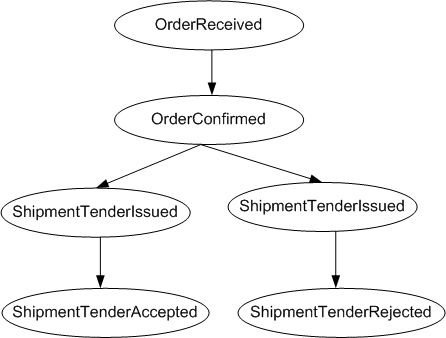
\includegraphics[width=0.7\textwidth]{pics/acyclicEventGraph.jpg}
	\caption{Directed acyclic graph of an event history}             
	\label{fig:dag}
\end{figure}  
%**********************
Martin Flower is addressing another important issuse regarding timing [http://martinfowler.com/eaaDev/TimePoint.html]. Date and Time information can come in different  precision formats. You could get a date on a daily precision and you could get it on msec precision level depending on your application. But as you work with events collected from different sources this could become a problem especially in distributed environments over the Internet where different time zones come in too. Furthermore the question arises which event occurence do you count? The one where the event happened physically on a machine or when it has been processed somewhere else? This kind of questions have to be considered when building a system to process or collect events from different distributed sources.
\\\\ 
In general a \textbf{causal relationship} determines that an event A caused another event B. As we have seen in our layered enterprise according to [Luckham05] events flow through these layered environment triggered by the user or another system at the top level and consequently transformed into lower level events down to the bottom causing other events to fire. This event flow is called \textit{vertical causality} and tracks down how high level events beginning from the business level manifest in lower layers. This is important to understand how these events are decomposed the way down in ordered to be able to create meaningfull aggreagations out of the masses of low level events. On the other hand Luckham talks about \textit{horizontal causality} that tracks the causal relationships between events at the same level. Causal relationships are transitive and asymmetric and can be represented as directed acyclic graphs. 
\\\\
\textit{Recognizing or detecting a siginificant group of lower-level events from among all the enterprise event traffic, and creating a single event that summarizes in its data their significance, is called event \textbf{aggregation}.} [Luckham05]
\\\\
Aggregating events is a difficult tasks as it needs a technology that can recognize patterns of events through different layers. But if such an aggregation facility is set up and running it can be a powerful source of tracking down causalities between events.

%**************************************************************************************
\subsection{Eventbased systems}
%**************************************************************************************
The term of event-based systems is used in many fields in an ambigious and varying way. As we have decribed several messaging architectures like the persistent, transient and asychronouse way to deliver messages to a client there is a distinct line between simple message exchange and event-based systems. The exhaustive trend of using distributed system architecture to support highly automated data processing has led to the concept of client-server architectures that brough major drawbacks with it. A classic client-server architecture, where system compontents access remote functionality to acomplish their own tasks, is often a synchronouse communication between the server and the client. That leads to tight coupling and affects the scalability of such architectures. Several middleware extensions addressed this problem by allowing to use asynchronous messaging in an either persistent or transient way using the mentioned message queing techniques. 
\\\\
In an event-based environment we have components communicating with eachother by sending and receiving event notifications. There are mainly two interacting components the \textit{consumer} and the \textit{producer}. The consumer is subscribing to certain notifications and the other component, the producer, is publishing notifications about various topics. A notifications service dispatches the notifications from the producer to the subscribed consumer. This notification service makes it possible to create easily loosly coupled and scaleable infrastructures as none of the components have to know about eachother. The notifications itself is created by observing special occurrences that are a point of interest. The subscription of consumers is a list of certain notifications the consumers wants to receive by the notification services. The subscription mechanism could be just a filter function or a more sophisticated notification selection mechanism including metadata descriptions. A channel would represent such a bundle of notifications that a consumer could subscribe and a producer could select to distribute its notifications.
\\\\
%**********************
\begin{figure} [ht]                
	\centering                                           
	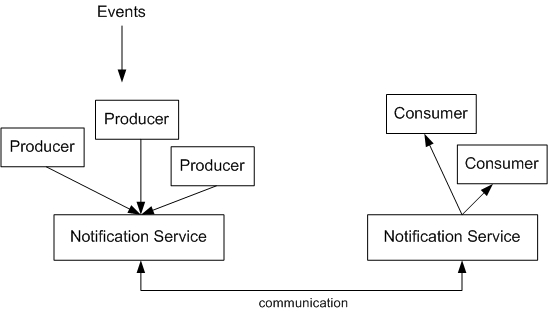
\includegraphics[width=1\textwidth]{pics/eventBasedConsumerProducer.jpg}
	\caption{Event-based notifications}             
	\label{fig:event-basedNotifications}
\end{figure}  
%**********************
\\\\
As you can see there is the major drawback of missing filtering, aggregation and colleration services like mentioned in the introduction. Actually there is no big deal to set up a message queue for a component or a system to receive specific event notifications from a channel. Let assume that you have a component or a system subscribed to a shipment tracking channel that sends continouse notifications about the current status of a package and another subscription to a channel that notifies about shipment audits. The system would be able to handle those received events according to its assigned tasks in ways like: 
\begin{itemize}
	\item \textit{The shipment xy has been audited and a damaged product has been indentified.} The system can book product xy from shipment xy as damaged.
	\item \textit{The shipment xy has been delivered.} The system can book the shipment xy as finished.
	\item \textit{The shipment xy is currently on road between Vienna and Linz.} The system can react in sense that it updates a some location tracking systems used.
\end{itemize}

There is a wide range of options how to deploy systems even in ways that systems can react in very intelligent ways, but in sense of gathering high level business information or tracking business processes it won't be possible as you would need a facility that collects all events and it would even need access to historic data in some cases to find out for example what caused to failed the shipment from the example above. If you would want to create high level overviews of that shipment you would need correlation information about those events that belong to one shipment or you would need aggregation functionality to create more abstract groupings of those information. Another problem dimension is that todays business environment requires a fast paced  decision infrastructure based on up-to-date information. For long people complied with that decision making does not require actual data instead it needs huge amounts of historical information collected in data warehouses. 
\\\\
\textit{[...] strategic decision makers are being exposed to the huge inflows of data and information from their resources and they are under rigid time constraints to make the right decisions.} [NguyenSchieferTjoa05]
\\\\
According to Hackathrone the business value of taking an action goes down after an event happend (see Figure \ref{fig:event-basedNotifications [Hackathorn02]}).

%**********************
\begin{figure} [ht]                
	\centering                                           
	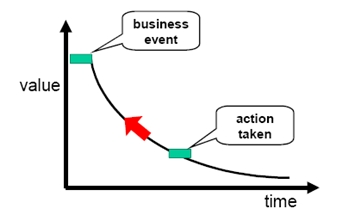
\includegraphics[width=0.8\textwidth]{pics/businessValue.jpg}
	\caption{Event business value}             
	\label{fig:event-basedNotifications [Hackathorn02]}
\end{figure}  
%**********************
%**************************************************************************************
\subsection{Related work to event-based systems}
%**************************************************************************************
Currently there is quite a lot of work going on in the design and application of event-based system support and correlatin systems. This chapter will introduce some of the most prevalent systems.

%**************************************************************************************
\subsubsection{Senactive InTime - Sense and Response Architecture}
%**************************************************************************************
%**********************
\begin{figure} [ht]                
	\centering                                           
	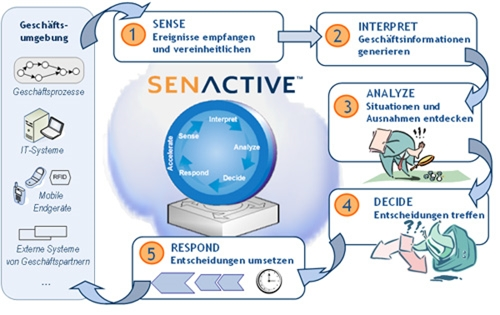
\includegraphics[width=1\textwidth]{pics/senseAndResponseSenactive.jpg}
	\caption{InTime Sense and Response Architecture \cite{SenactiveWebpage}}             
	\label{fig:senseAndResponseSenactive}
\end{figure}  
%**********************
The basic idea behind the \textit{Sense and Response Service Architecture} used in Senactive's InTime product is to monitor IT- and businessprocesses in sense and response loops. This architecture allows to gather business intelligence data and make decisions based on actual information. Real-time event sources are connected to the system by event adapters and fed into \textit{Sense and Response loops} which is divied into 5 phases. 
\\\\
The 5 phases in detail (see Figure \ref{fig:senseAndResponseSenactive}) \cite{NguyenSchieferTjoa05} :

\begin{itemize}
	\item \textbf{Sense}: Continouse capturing of of events and unification by the sense and response architecture.
	\item \textbf{Interpret}: The events will be transformed into business information like performance indicators, business situations and exceptions.
	\item \textbf{Analyse}: Analysis of interpreted business information to preditct performance and risks if the business environment changes.
	\item \textbf{Decide}: Proposal for the best business situation and the accroding actions to be done either automated or by involving humans.
	\item \textbf{Respond}: Communicating the decision made in the last step to change the business environmant.
\end{itemize}

The processing, transformation and the relationshipdefinition steps can be defined for every organisation using an event processing model for modeling these sense and response loops.
\\\\
The system is capable of detecting exceptional business situations and can react on them by generating warnings or take measures by itself to prevent damages like fraud. The InTime product is also capable of correlating events and aggregating events from it's various sources. This product would help customers to monitor their event-driven enterprise systems from a high level perspective to gather financial ratios, to trace down occured problems or to use it for decision making based on real time information. As this product can react proactivly on given business situations in its \textit{decide cycle} it can change business situations autonomously based on rules and provided information. The change of business situations can be performed in an event-based manner again. 
\\\\
This \textit{Sense and Response Service Architecture} can be used to satisfy real-time business intelligence architecture requirements as it can be used as a real-time data cache that serves as a staging area for datawarehouse updates and analytical services. More on zero-latency data warehousing and real-time business intelligences has been addressed here \cite{TjoaNguyenKickinger04}, \cite{NguyenSchieferTjoa05} and \cite{ThoManhNguyen05}.
\\\\
A useful feature of Senactives InTime is an event simulator that can generate events to create simulations to test event workflows or to generate event-based data for other purposes. This feature has been used for this diploma thesis to simulate logistics service prodiver based upon some special exceptional stories created. 

%**************************************************************************************
\subsubsection{RAPIDE}
%**************************************************************************************
RAPIDE is an event pattern language developed at Stanford University by the Program Analysis and Verification Group under the lead of David Luckham. RAPIDE is a declerative computer language that enables the specification of patterns of events. The syntax of of RAPIDE is basically like todays languages like Java or C\#. RAPIDE allows the specification of patterns that form relationships between events by causal, content or temporal constraints. This language has the feature to add pattern rules during runtime while events are collected according to the given pattern rules and processed by given action statements. Rapide is capable of aggregating high level events out of a collection of correlated events.
\\\\
It has a rich set of features \cite{Luckham05} like:

\begin{itemize}
	\item Definition of Event types.
	\item Event pattern definition
	\item Pattern operators for modeling relationships between events.
	\item Temoral operators to specify the timeing of events.
	\item Pattern macros for building more complex patterns.
\end{itemize}

According to \cite{LuckhamManensPark} RAPIDE is a good approach to test and simulate business process as it is easily possible to track causal relationships and to detect contraint violations during simulation. 

%**************************************************************************************
\subsubsection{Generalized Event Monitor - GEM}
%**************************************************************************************
%**********************
\begin{figure} [ht]                
	\centering                                           
	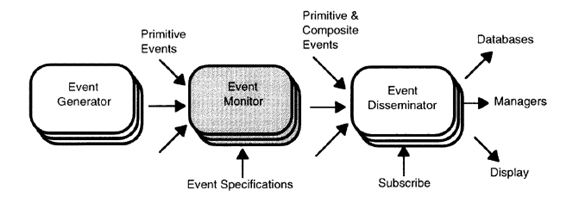
\includegraphics[width=1\textwidth]{pics/GEM.jpg}
	\caption{Event monitoring components \cite{GEM95}}             
	\label{fig:gemEventMonitoringComponents}
\end{figure}  
%**********************
The Generalized Event Monitor (GEM) is an interpreted declarative rule-based event monitoring language which allows to specify high-level events out of different nodes in a distributed system. The purpose of GEM is to monitor operations of distributed systems to support managment decisions and control network behaviour. The monitor is capable of applying filters and to correlate events according to predefined rules. GEM's pecification contains the type of the vents to be collected, a pattern that has to be matched and an action to be performed. GEM's specification is very powerful as it allows the definition of triples (format, composite event definition and actions to be defined). Moreover it is possible to modify the GEM monitors state. The main drawback is that it does not support to model causal relationships between events which result in a lack of defining patterns based on causalities between events. For further details see \cite{GEM95}.
%**************************************************************************************
\subsubsection{HP-ECS Event correlation service}
%**************************************************************************************
%**********************
\begin{figure} [ht]                
	\centering                                           
	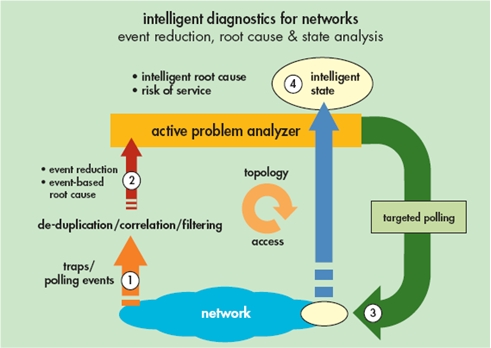
\includegraphics[width=1\textwidth]{pics/openView.jpg}
	\caption{HP-ECS OpenView \cite{OpenViewHP}}             
	\label{fig:openViewHPECS}
\end{figure}  
%**********************
Hewlett Packard provides a commerical event correlation product for correlating events coming from various system levels like the lower network layers, enterprise systems and application or database systems. HP-ECS correlates events by defineing correlation circuits either with a sophisticated GUI. These correlation circuits are a set of nodes connected to each other where the events pass through.  
\\\\
Events can be passed through intermediate nodes in a circuite that provides different features like:
\begin{itemize}
	\item temporal filters
	\item causal filters
	\item content filters
	\item in general event monitoring
	\item sequential event contructs 
\end{itemize}

HP-ECS has a major flaw because it is not usable for generic event correlation as it only supports correlation for SNMP and CMIP events.

%**************************************************************************************
\section{Scope of this diploma thesis}
%**************************************************************************************

We have seen in the previous chapters which impact events have got in todays decision making processes and what value it creates for process managment especially in large and global oriented enterprises. E-Business and E-Markets have created a global playground for automated workflow systems which results in a huge traffic flow of information between corporate networks and department systems. The lack of monitoring these events in a sense of correlating them, creating causal relationships or aggregate them to high level events is still a problem that is currently challenged by academic and commerical oriented institutions. Some of them like Senactive's Sense and Response Architecture provides the ability to monitor event flows and proactivly react on them to change the business processes based on real-time information provided by the various enterprise systems. This is a major step towards real-time enabled enterprises that can challenge the requirements of todays highly dynamic business world. 
\\\\
The core of this diploma thesis does not go in first place into event-based processing problems like creating sophisticated causal trackings or correlation algorithms. This thesis is about a system that enables the historic view of collected historic event streams that have been preprocessed by Senactives InTime Sense and Response Architecture. As Intime can react proactivly on given business situations based on event constellations and defined rules it can rearrange business processes to stear the business environment and processes into a given direction. This will result in a chain of newly triggered event flows which join back to the control loop. InTime is capable or correlating events according to predefined rules and delivers causal tracking of events. 
\\\\
The system developed in this diploma thesis is collecting those \textit{catched} events and creates a full text index over them to enable a Google like search experience for investigation purposes. The major application of this system is to offer the user a toolset to discover different aspects of business processes based on event correlations. This system has evolved over several stages to clarify which architecture would be the best solution to provide this kind of search and discovery experience to a user and at the same time to lay the foundation for further work in the area of event mining and correlation discovery. 

%**************************************************************************************
\section{Information Findability}
%**************************************************************************************
According to \cite{Morville05} findability is described by following aspects:

\begin{itemize}
	\item \textit{The quality of being locatable or navigable.}
	\item \textit{The degree to which a particular object is easy to discover or locate.}
	\item \textit{The degree to which a system or environment supports navigation and retrieval.}
\end{itemize}

Google has shown the world that searching the web does not have to be based on simple keyword matchings or word frequency countings. It introduced a completle new way of rating weppage contents and to calculate the best hits out of some search terms provided by the user. Google's commercial success has proven the world that this way of finding information is the right one at least for the moment as long as noone else comes with a better idea. 
\\\\
The look and feel of Google like finding and retrieving information has become a defacto standard and numerous applications integrate full text indexing algorithms and methods into their applications to provide a search based access to information and data. These applications don't necessarliy concentrate on finding webpages it's applied on a variety of information like office documents, products, flight schedeules or even free available source code. People tend to go away from the classic topologic of classifying information into tree like catalogous and let the user to navigate through these structures to get their desired information. A good indexing and retrieval mechanism allows the users to find and access information by typing some terms into a textbox and a ranking algorithm calculates the best hits out of the found information to present the most relevant information. This way of organising the access to information has become a great success as numerous applications has proven like koders.com, Google Desktop Search and Apple's Spotlight for instance. 
\\\\
\textit{Of course, access doesn't simply require us to make decisions in more areas of our lives. It also changes the game by inviting us to make informed decisions more often.} \cite{Morville05}

%**************************************************************************************
\subsection{Event Cloud Background}
%**************************************************************************************

% welchen bedeutung hat event cloud? siehe scope
% was kann der Benutzer damit machen?
% Grundlage f�r Eventmining und correlation finding
% Geeignete Architektur f�r so eine Anwendung finden
% Fokus auf freie Technologien

Event Cloud is the name of the developed application whose main purpose is to provide a search interface to its users to allow them to search for simple and correlated events in an efficient way.  The representation of the search results is a major feature that allows its user get the most relevant hits according to the given search criterias. Furthermore it provides functions to exclude unwanted event and correlation types from the found result set and it allows to create filters over events and their correlations. As not every person is interested in all types of occured events and correlationsets it is possible to create and edit roles for different user profiles that will reduce the information pool to a desired managable pool of events and correlations. Event Cloud provides the user the option to to dig down to event levels or to go up to correlation levels according to the selection from a found resultset. 
\\\\
Basically Event Cloud has implemented two Search types that allows a user to query for either events or to search through whole event correlations. Using the latest Java high-performance text search engine library Lucene and the powerful open source database Postgres allows to index and search the event repository in a fast and efficient way. The system is supported by the lightweigt IoC Spring framework to bind the components together. A special focus has been set on using only non-proprietary and open source technologies as this an academic project and should lay the cornerstone for future work on this topic or at least provide useful information how to do or not to do future work in this field. 
\\\\
Basically Event Cloud consists of three main functions: 

\begin{itemize}
	\item Extracting and transforming event data from the source system and integrate them into Event Cloud's own data structure.
	\item Full text index over simple and correlated events.
	\item Search functionality including a sophisticated query syntax and various filter functions
\end{itemize}

These functionalities should provide a powerful toolset to facilitate the discovery of different aspects of business processes based on event correlations provided by a Google like search experience. 
\\\\
This diploma thesis was especially supported by Josef Schiefer and Senactive by providing InTime for the basic infrastructure and support throughout the whole developing process. Especially the simulation of business processes to gather test data in form of generated events was done by the InTime product. Plenty of time has been invested to create interesting and meaningful simulations of business procesess based on a logistics company. The event simulation has been broadend by according stories for showcases to display exceptional situations and to show how InTime can react on such situations. The simulation definition process has been co-developed by Roland Vecera and is available as an Appendix in the diploma thesis to get a comprehensive view of what happens beneath the fact that events exits for this project.
\\\\
As we talk about source systems or the source database throughout the next sections it is always the InTime database meant. This is a Ms Sql Server database that contains the raw event information from the InTime simulator. As InTime is settled in the .Net world, Event Cloud provides an import functionality to duplicate the database on a desired machine as usually InTime has been deployed in a VMWare for developing purposes which is not a performance wonder.

%**************************************************************************************
\newpage
\subsection{Search Concepts}
%**************************************************************************************
% Das Suchen ist der zentrale Teil daher muss man bestimmte Suchkonzepte unterscheiden die
% vom System unterst�tzt werden.
The subsequent chapters will give an conceptual overview of the search type features provided by Event Cloud. These are the basic concepts behind the Event Cloud and no further technical details are provided in this section.

%**************************************************************************************
\subsubsection{Rank 1}
%**************************************************************************************
The Rank 1 search is simple full text search over all searchable attributes of an event. The user is able to put down a search query consisting of several search terms and boolean operators according to Lucenes BNF query syntax. The result will be a list of events that matched the given query. 
\\\\
The Rank 1 search is pretty straight forward like you would search documents on the internet using any search engine available. 
\\\\
Take a look at the example (Figure \ref{fig:rank1searchExample}) where we have several events in our repository. The user queries for the terms "Paris London Szabolcs" and gets back the events TransportEnd and TransportStart as these terms occured in those events ordered by the most relevant hits. No boolean operators have been applied in this query example. If the user would have entered a query like "szabolcs AND Paris" he would have received events where the terms Paris and Szabolcs would have occured. For more details take a look at the query syntax as this is not in the scope of this chapter.
%***********************
\begin{figure}[ht]                                  
	\centering                                           
	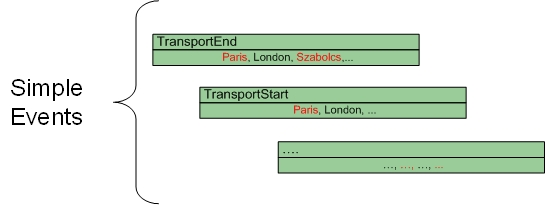
\includegraphics[width=1.0\textwidth]{pics/rankOneSearchExample.jpg}
	\caption{Rank 1 search example}             
	\label{fig:rank1searchExample}
\end{figure}            
%***********************      
%**************************************************************************************
\subsubsection{Rank 2}
%**************************************************************************************
At the current point the heart of Event Cloud is the Rank 2 search which is an extension of the Rank 1 search. The difference between Rank 1 and Rank 2 search is that this search type is not looking at events at an atomic level rather it searches over whole correlations of events (Figure \ref{fig:rank2correlation}). By executing a Rank 2 search the query will go over whole correlationsets of events instead of looking only at events like in the Rank 1 search type. 
\\\\
%***********************
\begin{figure}[h]                                  
	\centering                                           
	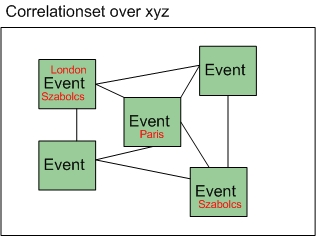
\includegraphics[width=0.7\textwidth]{pics/rankTwoSearchExample.jpg}
	\caption{Rank 2 search example}             
	\label{fig:rank2searchExample}
\end{figure}            
%***********************   
If a user puts down a search query consisting of terms like "Paris London Szabolcs" the search engine will retrieve correlations consisting of events that matched these terms (Figure \ref{fig:rank1searchExample}). That means that you will get back a correlation whose event attributes contain either Paris, London or Szabolcs. Correlationsets whose Events would not contain the terms "Paris London Szabolcs" would not be considered. If for instance a correlationset is consisting of eigth events and only one event contains the search terms it would be still a hit but maybe a bad one depending on the other found hits.
%***********************
\begin{figure}[h]                                  
	\centering                                           
	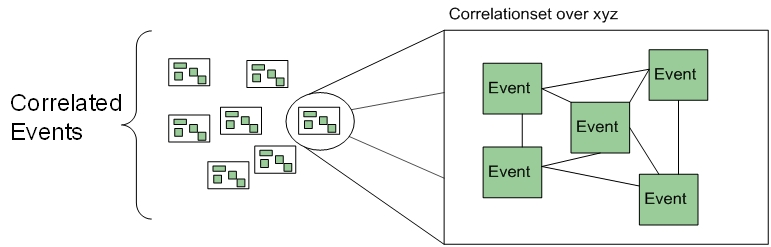
\includegraphics[width=1.0\textwidth]{pics/rankTwoCorrelation.jpg}
	\caption{Event correlation}             
	\label{fig:rank2correlation}
\end{figure}            
%*********************** 
   
%**************************************************************************************
\subsubsection{Rank 3}
%**************************************************************************************
This type of search is not implemented in the current work as it is a very complex topic and beyond the scope of this diploma thesis. For the sake of completness I want to give a brief overview about this event search type. The Rank 3 is searching over correlations like the Rank 2 search but instead of using direct correlations between events it searches over indirect correlations between correlationsets. It is actually the same like the Rank 2 but one aggregation level higher and the result hits are additionally evaluated by a distance factor of these indirect correlations.
\\\\
The challenge behind this type of correlation search is to discover indirect correlations between events and to implement an effective search alorithm to rank the most relevant hits. This technique could become a performance eating task as you have to find a way to consider a higher aggregation level when querying for events.
%***********************
\begin{figure}[h]                                  
	\centering                                           
	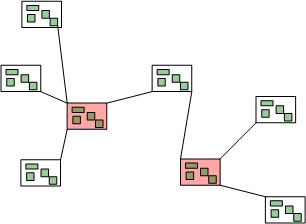
\includegraphics[width=0.5\textwidth]{pics/rankThreeSearchExample.jpg}
	\caption{Rank 3 search}             
	\label{fig:rank3searchExample}
\end{figure}            
%***********************  
%**************************************************************************************
\newpage
\section{Architecture}
%**************************************************************************************
% Hier fangen jetzt die Details an! High level Architektur + Technologien genau beschreiben
% High Level overview mit Bild und kurz die Komponenten beschreiben und wie sie zusammenspielen
% simulator f�r eventsimulation kurz erw�hnen und details dann beim Simulator abschnitt selber schreiben.
Event Cloud is a webbased application based on the lightweight Spring Framework IoC container and is deployed inside Apaches Tomcat. The core technologies for O/R Mapping and Indexing/Searching are Hibernate and Apache Lucene (Figure \ref{fig:eventCloudHighLevel}). 

% !!!!!!!!!!!!!!!!!!!!!!!!!!!!!!!!!!!!!!!!!!
% TODO: System layering!! siehe OSWP!!!
% !!!!!!!!!!!!!!!!!!!!!!!!!!!!!!!!!!!!!!!!!!

%**************************************************************************************
\begin{landscape}
%\subsubsection{High level overview}
%**************************************************************************************
%***********************
\begin{figure}[ht]                                  
	\centering                                           
	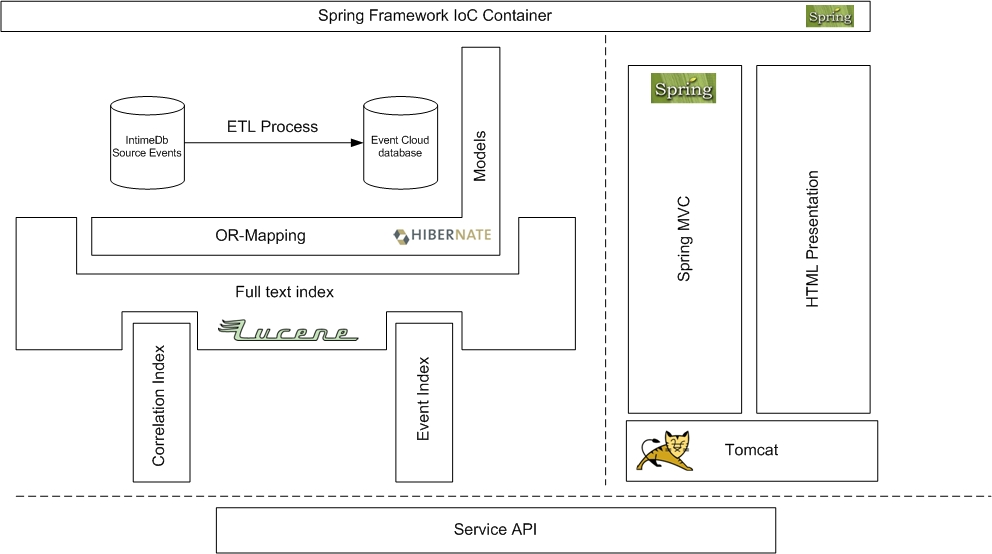
\includegraphics[width=1.2\textwidth]{pics/EventCloudHighLevelOverview.jpg}
	\caption{Event Cloud High Level Overview}             
	\label{fig:eventCloudHighLevel}
\end{figure}            
%***********************                       
\end{landscape}

%**************************************************************************************
\subsection{Database and Schemas}
%**************************************************************************************
There are two databases used by this system. The first one is the source database provided by InTime which contains the raw source events and the found correlationsets for those events. This is an Ms SQL Server database that requires the sqljdbc drivers in order to establish a connection from hibernate. As the second database there is a currently a Postgres 8.1 database in use as it is open source and a powerful technology that fits the needs for this project. However using Hibernate as the O/R mapping facility it is possible to change the database backend with only minor changes. Only sequence definition changes have to be done at the mapping level as Postgres is using sequence tables for id generation. The source schemas are pretty straight forward flat tables (Figure \ref{fig:intimeschema}) and the final target schema created out of the source events is bit more complex as Event Cloud decomposes the events and stores them into a relational form (Figure \ref{fig:eventCloudSchema}). 
\\\\
%***********************
\begin{figure}[h]                                  
	\centering                                           
	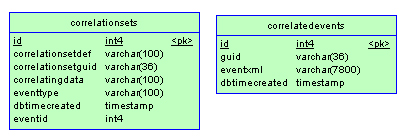
\includegraphics[width=1.0\textwidth]{pics/intimedb.jpg}
	\caption{Intime schema}             
	\label{fig:intimeschema}
\end{figure}            
%***********************
The rwtime and txtime tables represent the realworld dates of events (rwtime) e.g. when they really occured in some system.  The timepoint when events have been recognized by the system are decomposed and stored in the txtime table. During the ETL process the event timestamps are decomposed to a day, month and year granularity. The rwtime and the txtime tables hold every possible combination of day, month and year as the event numbers grow and only the ids are assigned to the event. This allows an efficient indexing of the dates and thus a fast way to create constrained date queries.
\\\\
The events and eventattributes relations are the core tables in the target schema of Event Cloud. Basically the event relation holds the core event information provided by each event. The eventattributes relation holds every extracted attribute from an event, its value and its unique URI as events are constructed out of XMLs that can get a complex structure. The logical XML strucuture is flattend in the relational form but to preserve the original substructures a URI is required. 
\\\\
Consider for example the mentioned OrderReceived Event (Listing \ref{lst:OrderReceivedEvent}) where you have got basic information provided with a Productcollection containing a subtree of several products. 
\\\\
A representation in the eventattributes relation would look like provided in Figure \ref{fig:OrderReceivedInEventattributes}.
%***********************
\begin{figure}[h]                                  
	\centering                                           
	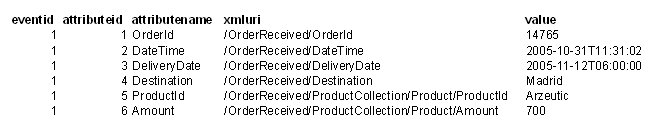
\includegraphics[width=1.2\textwidth]{pics/OrderReceivedInEventattributes.jpg}
	\caption{OrderReceived in eventattributes}             
	\label{fig:OrderReceivedInEventattributes}
\end{figure}            
%***********************  

The relation dbinfo is used to some information about the loading process and profiles is used to store profile information about filters for the search functionality.

The Index functionality of Postgres is a vital function that has been applied to the Even Cloud schema in Postgres to boost up performance. The standard index type of Postgres is a btree index which fits the needs as it can handle equality and range queries. As Hibernate does not support the creation of indexes it has to be added manually if the system is set up. An index can be created by using psql interface or antoher sql postgres access using the convention in listing \ref{lst:CreateIndexForGeneric}. 
\begin{lstlisting}[caption=Create an index, label=lst:CreateIndexForGeneric]{Create an index}
CREATE INDEX tablename_attributename_index 
	ON tablename (attributename);
\end{lstlisting}
Once the index has been created it will be updated automatically, but VACUUM ANALYSE has to be executed in regular intervals to update statistical data for the query planner. This has to be done especially when big amounts of data have been inserted into the database. Regular analysis can be executed by creating cron jobs over night for instance. 
\\\\
VACUUMing is important as rows are not physically deleted by Postgres if they are removed so this is necessary to reclaim storage space. VACUUming can be performed while reading and writing to tables as no lock is obtained but it will need some performance while running. 
\\\\
At this point it should be mentioned that Postgres is capable of handling different sorts of indexes found in \cite{PostgresDoc06} like partial indexing which could be useful to index only a subset of data stored in a table. This can be done by creating an index with a WHERE clause to specify the desired dataset. 
\\\\
Indexes are set on relation attributes according to Table \ref{tab:indexedAttributes}.

\begin{table} [h]
	\begin{tabular}{ll}
	 \textbf{Tablename} &  \textbf{Attribute} \\
	
	   	dbinfos &         id \\
	
		eventattributes & attributename \\
		
		eventattributes &    eventid \\
		
		eventattributes &      value \\
	
	 	eventtype & eventtypeid \\
	
	    rwtime &      rwday \\
	
	    rwtime &    rwmonth \\
	
	    rwtime &     rwyear \\
	
	    txtime &      txday \\
	
	    txtime &    txmonth \\
	
	    txtime &     txyear \\
	\end{tabular}  
	\caption{Indexed Attributes}
	\label{tab:indexedAttributes}
\end{table} 
     
%***********************
\begin{figure}[h]                                  
	\centering                                           
	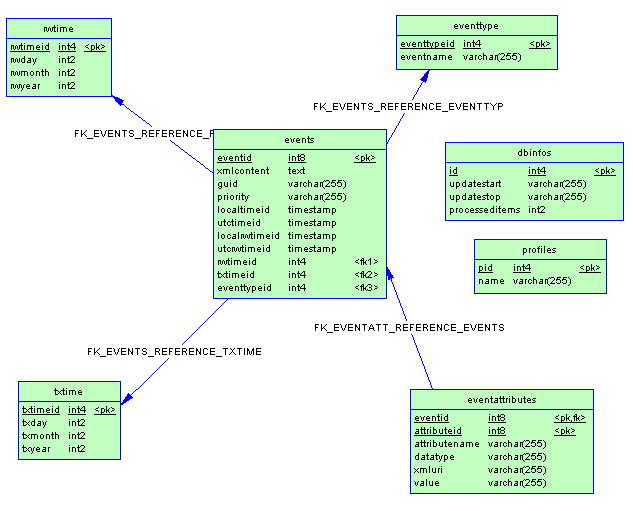
\includegraphics[width=1.0\textwidth]{pics/genericdb.jpg}
	\caption{Event Cloud schema}             
	\label{fig:eventCloudSchema}
\end{figure}            
%***********************     


%**************************************************************************************
\subsection{Object Relational Mapping}
%**************************************************************************************
We have seen in the previous chapter that the event sources and the transformed events are stored into relational databases. The whole data structure is based on a relational modeling paradigm which has proven itself over many years. The relational database technology has been originally introduces by E. Codd out of growing needs to structure data under specific standpoints and his works influence is still noticable. Almost every application needs a way to make its data persistent after shut down so a variety of products emerged over the years to provide a persistent and structured way to persist application data.
\\\\
Codd firstly introduced the relational model in his paper "A Relational Model of Data for Large Shared Data Banks": 
\\\\
\textit{It provides a means of describing data with its natural structure only--that is, without superimposing any additional structure for machine representation purpose. Accordingly, it provides a basis for a high level data language which will yield maximal independence between programs on the one hand and machine representation on the other.} \cite{Codd70} 
\\\\
A relational database is mainly characterized by of following terms \cite{Codd99}:
\begin{itemize}
	\item data independence from hardware and storage implementation
	\item automatic navigation
	\item nonprocedural language for accessing data
\end{itemize}

This had a big impact and changed the way how data has been processed. Instead of manipulating record by record it was possible to describe the datasets for processing and to store data in an efficent way. Today a database managment system is more than a formal description of how to organise and structure information. It provides a full blown information managment system that allows applications to access large amounts of data in a fast manor. It supports transactions, user managment, issues security topics and much more. Moreover the relational world has been and is still under academic discussions which helps to evolve the algorithms and technologies powering those technologies. A lot of work has been invested to mathematicaly formalize relational model and to develop a structured query language. Currently there is a wide range of commercial and open source database managment systems available like DB2, Orcale, Ms SQL Server, MySQL or PostgreSQL.
\\\\
As time goes by people realized that procedureal programing paradigms create too much overhead which makes systems difficult to maintain, components hard to reuse and the world could be described in better ways for problemsolving. As a result the object oriented paradigm has evolved and Smalltalk was the first noticeable programming language that introduced the object oriented programming paradigm together with cutting edge features (at least for that time). During the mid eighties C++ established the object oriented paradigm into eveybodies minds. Programming languages evolved over time and todays most widely spread languages are C++, Java and .Net derivates. Especially Java has proven itself for developing distributed applications. Today we have a sophisticated toolset available like modelling languages such as UML or a rich set of design patterns for different purposes we can use more or less out of the box (for more details take a look at \cite{DesignPatterns97} and \cite{Fowler97}).
\\\\
Today we are facing the problem of a \textit{paradigm mismatch}. We started to use object oriented techniques to model and develop our applications, but almost all of our  systems have the requirement that they need to persist their data. Following the object oriented paradigm we create domain models about the subjects we need to work with. Sometimes these models are named business models in a layered application context. This object oriented style of modeling our data clashes with the well known relational \textit{row and column world}. The problem is that object oriented domain models are simply the better choice as it helps to improves code reuseability and the maintainability significantly. 
\\\\
The first approaches that addressed this problem were to create sql support to enable a link between the relations stored in a database and the business models to benefit from their advantages. This approach is very expensive as the developers have to write low level SQL statements using database APIs into the source code directly not to speak about the almost unchallengable task to implement sophisticated algorithms like lazy-loading of object graphs that represent 1:n relations in a relation model or caching techniques to improve performance. You never would have thought about changing the database at the back end of such an implementation and even a schema change can get out of hand. Developers face huge problems that don't belong to the given business domain problem at all in order to create a clean and object oriented application.
\\\\
The solution to this problems is the object relational mapping (ORM) approach that keeps the developers away from the underlying persistence mechanisms. Developers only need to create a persistence layer that declerativly wires the business models to their relational counterparts. The underlying persistence mechanism does the rest for the developer including sophisticated techniques to boost performance for instance.
\\\\
\textit{In a nutshell, object/relational mapping is the automated (and transparent) persistence of objects in a Java application to the tables in a relational database, using metadata that describes the mapping between the objects and the database. ORM, in essence, works by (reversibly) transforming data from one representation to another.} \cite{HibernateInAction05}
\\\\
The main features provided by ORM approach are:
\begin{itemize}
	\item It shields developers from low level sql coding.
	\item It let the developers concentrate on bussiness problems.
	\item It reduces development time significantly.
	\item It produces less lines of code that makes understanding a system and refactoring easier.
	\item It is database independent.
\end{itemize}
There are several ORM libraries available. For this project the decision has been made to use Hibernate, because it is wide spread and meanwhile a rock solid Java library with big support community. It was important to keep the database technology out of scope in this project. Although the decision has been made to use Postgres for Event Cloud we wanted to keep the option to deploy other database technologies. Another important fact is that Hibernate has an outstanding performance as it creates almost no overhead and is able to make use of sophisticated caching mechanisms.

%**************************************************************************************
\subsubsection{Data access object}
%**************************************************************************************

Event Cloud uses the Spring Framework to manage the components of this application by applying the Factory Pattern, IoC and code injection. More on this topic later on. What's important is to be aware of, that the Spring Framework is taking over a lot of work handling Hibernate and data access. Spring supports declearive definition of the Factory pattern and a dependeny injection.
\\\\
The Spring Framework brings a Data Access Object (DAO) support with it that is applied in Event Cloud. The idea behind DAO is to follow object orieted principles and thus to programm agains interfaces. You define a DAO interface and a concrete implementation of this DAO. The application now can access the DAO interface through higher level services (Figure \ref{fig:DAOconcept}). Spring binds the DAO implementation to the interface. This enables a loosly coupled design, improves maintainability and speeds up testing processes. Moreover the DAO pattern has the advantage that is easily possible to change the underlying data access even much faster.
\\\\
%***********************
\begin{figure}[ht]                                  
	\centering                                           
	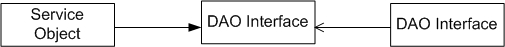
\includegraphics[width=1.0\textwidth]{pics/DAOConcept.jpg}
	\caption{DAO concept}             
	\label{fig:DAOconcept}
\end{figure}            
%*********************** 

%**************************************************************************************
\subsubsection{Integrating Data Access}
%**************************************************************************************

The Figure \ref{fig:SessionFactory} shows the basic wiring to establish database connections and integrate the data access into the application. The centerpiece of the data access in Spring Framework managed applications is the SessionFactory. The SessionFactory serves as a session factory for dependency injections on thread safe DAOs. Event Cloud uses the LocalSessionFactoryBean as a concrete implementation which is appropriate for most types of scenarios even to deploy distributed transaction support or JNDI support. It is all just a matter of configuration. For example if we would want to change the database connection to a JNDI resource we just change the LocalSessionFactoryBean implementation to JndiObjectFactoryBean and readjust the connection string. 
%***********************
\begin{figure}[h]                                  
	\centering                                           
	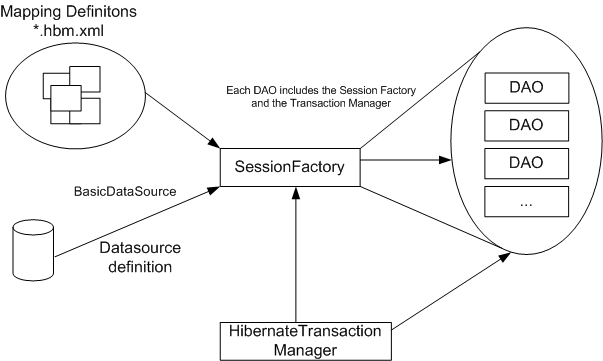
\includegraphics[width=1.0\textwidth]{pics/SessionFactory.jpg}
	\caption{Data Access integration}             
	\label{fig:SessionFactory}
\end{figure}            
%*********************** 
The listing figure \ref{lst:SessionFactoryConfiguration} shows a bunch of configuration options that have to be applied. Important note is to specify the SQL dialect according to you database managment system and create an injection link to you database connection bean (<ref bean="postgresSource"/>) which will be wired in by the Spring Framework. The hibernateProperties allow some finetuning options like caching options and switches to turn on and off to help debugging.
\\\\
%***************************************
\begin{figure}[h]  
	\begin{mytinylisting}
	\begin{verbatim}
	<bean id="sessionFactoryForPostgresSource" class="org.springframework.orm.hibernate3.LocalSessionFactoryBean">   
		<property name="dataSource"><ref bean="postgresSource"/></property>
        <property name="mappingResources">
            <list>
            	<value>Event.hbm.xml</value>
				<value>Rwtime.hbm.xml</value>
				<value>Txtime.hbm.xml</value>
				<value>Eventattribute.hbm.xml</value>
				<value>Eventtype.hbm.xml</value>
				<value>Dbinfo.hbm.xml</value>				
            </list>
        </property>
        <property name="hibernateProperties">
        <props>
            <prop key="hibernate.dialect">org.hibernate.dialect.PostgreSQLDialect</prop>
            <prop key="hibernate.hbm2ddl.auto">update</prop> 
			<prop key="hibernate.show_sql">true</prop>
			<prop key="hibernate.cache.provider_class">org.hibernate.cache.EhCacheProvider</prop>
        </props>
        </property>
    </bean> 
   	\end{verbatim}
	\end{mytinylisting}
	\caption{The data access heart the SessionFactory configuration}             
	\label{lst:SessionFactoryConfiguration}
\end{figure} 
%***************************************
An important property is the mappingResources as it defines the mapping resources for the application. The mapping resource files are ending with a *.hbm.xml by standard and they provide the mapping definitions between the relational and the object oriented world. Creating and parametrizing the mapping resources is far out of scope in this diplom thesis as there is an excellent documentation available on the Hibernate webpage. Important is that there are tools and techniques available that can generate these mapping configuration files for your application. In this project a top-down approach has been chosen to create data access. The idea is to create the relational database schema and define various contraints. The next step is to apply a tool name Middlegen which is capable to read in the database schema and provide a user interface to create the object relationl mapping resources. When this has been done a tiny program can be integrated using Jakarta's Ant to generate the object oriented models including object graphs for representing relationships. Afterwards all that have to be done is add the mapping resource names to the SessionFactory.
\\\\
The database connections are defined in the context defintions of the application. One for the target database, the Event Cloud, and one for the source database (see listing figure \ref{lst:DatabaseConnection}). As we have two databases another SessionFactory instance for the second database has to be created too. For means of simplicity there is only one example provided just to show how the basic concept works if changes have to applied and how this is all wired together. Event Cloud makes use of the commons pooling package to provide basic connection pooling for the application. I someone would like to use a more sophisticated implementation like C3PO it is again just a matter of changing the class. 

%***************************************
\begin{figure}[h]  
	\begin{mytinylisting}
	\begin{verbatim}
	<bean id="postgresSource" class="org.apache.commons.dbcp.BasicDataSource">
	  <property name="driverClassName"><value>org.postgresql.Driver</value></property>
	  <property name="url"><value>jdbc:postgresql://localhost/generic</value></property>
	  <property name="username"><value>postgres</value></property>
	  <property name="password"><value>postgres</value></property>
	</bean>
	\end{verbatim}
	\end{mytinylisting}
	\caption{Database Connection}             
	\label{lst:DatabaseConnection}
\end{figure} 
%***************************************


%**************************************************************************************
\subsubsection{Transaction Managment}
%**************************************************************************************

Now it comes an important topic: the transaction managment. Spring Framework supports a wide range of transaction managers and the transaction managment itself can be configured in a declerative way for each DAO and each method of the data access objects used in the application. Event Cloud makes use of the HibernateTransactionManager that is wired to the SessionFactory (Listing figure \ref{lst:TransactionManagment}). Note that this is a huge step! For long declerative transaction managment was only supported by EJB which had to be deployed inside heavy weight application servers with a wide range of drawbacks. The Spring Framework comes with declerative transaction support implemented through Spring's AOP framework. 
\\\\
%***************************************
\begin{figure}[h]  
	\begin{mytinylisting}
	\begin{verbatim}
	<bean id="transactionManagerForPostgresSource" class="org.springframework.orm.hibernate3.HibernateTransactionManager">
        <property name="sessionFactory">
        	<ref bean="sessionFactoryForPostgresSource"/>
        </property>
	</bean>
	\end{verbatim}
	\end{mytinylisting}
	\caption{Transaction Managment}             
	\label{lst:TransactionManagment}
\end{figure} 
%***************************************

The DAO, created by the user, references the previously defined SessionFactory and has to extend the HibernateDaoSupport. The TransactionProxyFactoryBean is used to enable the declerative transaction managment for a DAO. It needs three properties to be defined:

\begin{itemize}
	\item The transaction manager - in this case it is the HibernateTransactionManager
	\item The transaction target - this is a reference to the DAO that includes the SessionFactory
	\item The transaction attributes - decleares which type of transaction type to apply to which methods including options.
\end{itemize}

%***************************************
\begin{figure}[h]  
	\begin{mytinylisting}
	\begin{verbatim}
	<bean id="correlatedEventDAOTarget" class="at.generic.dao.hibernate.CorrelatedeventDAOHibernate"> 
    	<property name="sessionFactory"> 
    		<ref bean="sessionFactoryForSQLServer"/> 
    	</property> 
    </bean>
	
	<bean id="correlatedEventDAO" class="org.springframework.transaction.interceptor.TransactionProxyFactoryBean"> 
    	<property name="transactionManager"> 
        	<ref bean="transactionManagerForSQLServerSource" /> 
      	</property> 
		<property name="target"> 
		   <ref bean="correlatedEventDAOTarget" /> 
		</property> 
      <property name="transactionAttributes"> 
         <props> 
            <prop key="save*">PROPAGATION_REQUIRED</prop>
            <prop key="update*">PROPAGATION_REQUIRED</prop> 
            <prop key="remove*">PROPAGATION_REQUIRED</prop>
			<prop key="*">PROPAGATION_REQUIRED, readOnly</prop>
         </props> 
      </property>
    </bean>
	\end{verbatim}
	\end{mytinylisting}
	\caption{Integrating transaction managment for a DAO}             
	\label{lst:TransactionManagmentDAO}
\end{figure} 

The transaction attributes cover propagation rules and isolation levels that can be defined for each method. The key properties defines on which methods they should be applied. For example on methods starting with "save*" Propagation is required.
\\\\
Available propagation rules are PROPAGATION MANDATORY, ROPAGATION NESTED, PROPAGATION NEVER, PROPAGATION NOT SUPPORTED, PROPAGATION REQUIRED, PROPAGATION REQUIRES NEW and PROPAGATION SUPPORTS (detailed explanation is available here \cite{SpringInAction05}). Event Cloud mostly uses the PROPAGATION REQUIRED which will create a transaction for the methods. The read-only option is important to apply for attributes that perform only read operations as this option activates certain optimization options that may boost up the performance during such transactions. There are also five isolation levels available to set that are also described in detail here \cite{SpringInAction05}. These levels are ISOLATION DEFAULT, ISOLATION READ UNCOMMITTED, ISOLATION READ COMMITTED, ISOLATION REPEATABLE READ and ISOLATION SERIALIZABLE.

%***************************************

%**************************************************************************************
\subsubsection{Event Clouds Persistence Layer}
%**************************************************************************************

Event Cloud's data access is following the data access object (DAO) pattern using Hibernate and Spring Frameworks support described in the previous sections. For each database there are models generated using a top-down approach. The resource mappings between the relational database and the business objects or models are generated by middlegen and out of these mappings codegen generates the models according to their relational structure. 
\\\\
There are 8 model classes available that represent Event Cloud's target schema:
\begin{itemize}
	\item Dbinfo
	\item Event
	\item Eventattribute
	\item Eventtype
	\item Filter
	\item Profile
	\item Rwtime
	\item Txtime
\end{itemize}

And there are two model classes that represent Event Cloud's source schema from InTime:
\begin{itemize}
	\item Correlatedevent
	\item Correlationset
\end{itemize}
%***********************
\begin{figure}[h]                                  
	\centering                                           
	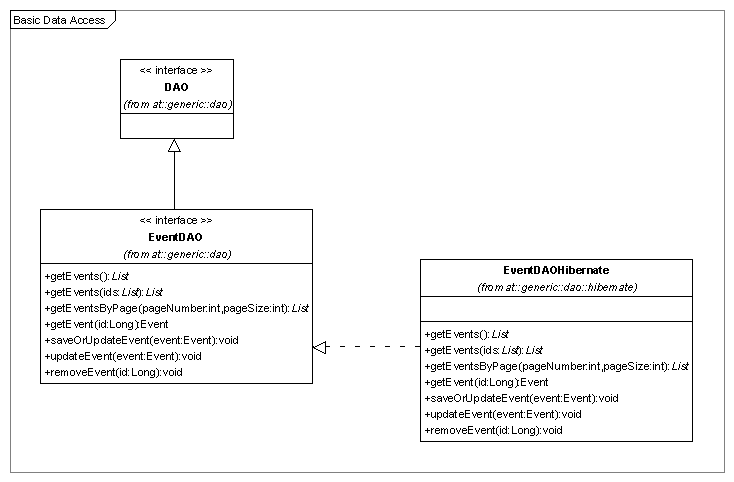
\includegraphics[width=1.0\textwidth]{pics/BasicDataAccess.png}
	\caption{Basic data access for events}             
	\label{fig:BasicDataAccess}
\end{figure}            
%*********************** 
For each of these models there is a DAO interface defined with basic CRUD (create, read, update, delete) methods. Some of them require special methods for different purposes. As the DAO interface is pretty forward there is no need to get into details here. The Spring Framework and Hibernate is doing all the all the hard work. The developer can concentrate on problems situated in the business domain.
\\\\
As Javadoc in combination with UML diagrams is self explainatory, I want to introduce only the basic concepts like the DAO for the for the event model (Figure \ref{fig:BasicDataAccess}). The DAO forms the central interface from where every other DAO interface is extended. The implementation of the EventDAO is Hibernate specific and is instantiated through Spring's context configuration (Listing Figure \ref{lst:ImplementingDAOInterface})

%***************************************
\begin{figure}[h]  
	\begin{mytinylisting}
	\begin{verbatim}
		<bean id="eventDAOTarget" class="at.generic.dao.hibernate.EventDAOHibernate"> 
		    	<property name="sessionFactory"> 
		    		<ref bean="sessionFactoryForPostgresSource"/> 
		    	</property> 
		</bean>
	\end{verbatim}
	\end{mytinylisting}
	\caption{Implementing DAO interface}             
	\label{lst:ImplementingDAOInterface}
\end{figure} 
%***************************************


%**************************************************************************************
\subsubsection{Persistence Service}
%**************************************************************************************

Event Cloud provides a high level API data access which encapsulates certain operations related to persistence. For example the EventPersistenceService extracts txtime and rwtime, eventtype data and transforms them into the appropriate models and stores them into the according relations using their DAOs. This helps other developers to use the service out of the box without to get into details about persisting events. 
\\\\
The EventPersistenceService is integrated by the Spring Framework using its contex configuration with dependency injection (Listing Figure \ref{lst:EventPersistenceService}). Like almost everywhere the EventPersistenceService also defined as an Interface whose implementation is wired in by the Spring Framework. 
%***********************
\begin{figure}[h!]                                  
	\centering                                           
	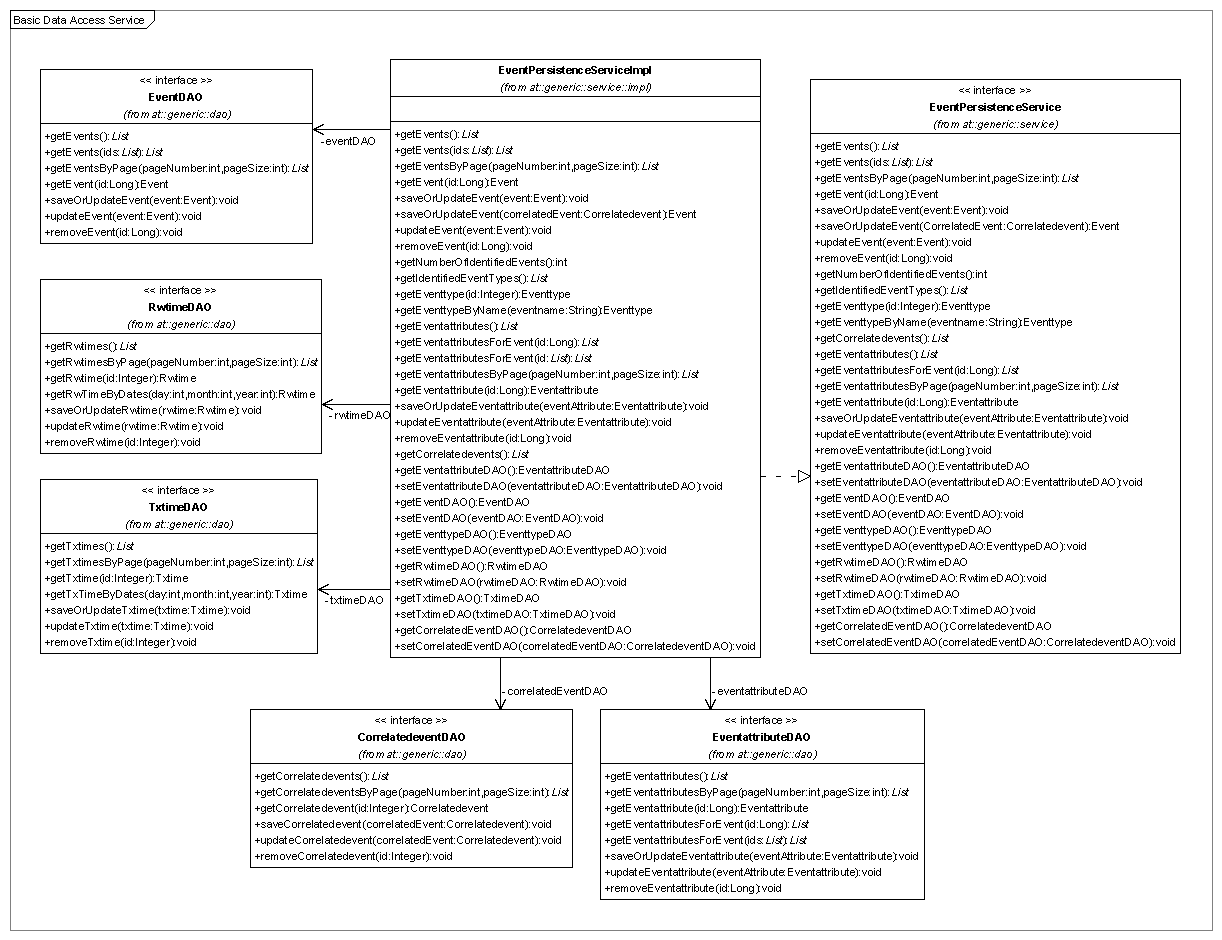
\includegraphics[width=1.0\textwidth]{pics/BasicDataAccessService.png}
	\caption{EventPersistenceService}             
	\label{fig:}
\end{figure}            
%*********************** 

%***************************************
\begin{figure}[h!]  
	\begin{mytinylisting}
	\begin{verbatim}
	<bean id="eventPersistenceService" class="at.generic.service.impl.EventPersistenceServiceImpl"> 
    	<property name="eventDAO">
    		<ref bean="eventDAOTarget"/>
    	</property> 
    	<property name="eventattributeDAO">
    		<ref bean="eventattributeDAOTarget"/>
    	</property> 
    	<property name="eventtypeDAO">
    		<ref bean="eventtypeDAOTarget"/>
    	</property> 
    	<property name="rwtimeDAO">
    		<ref bean="rwtimeDAOTarget"/>
    	</property> 
    	<property name="txtimeDAO">
    		<ref bean="txtimeDAOTarget"/>
    	</property> 
    	<property name="correlatedEventDAO">
    		<ref bean="correlatedEventDAOTarget"/>
    	</property> 
    </bean>
    \end{verbatim}
    \end{mytinylisting}
	\caption{EventPersistenceService}             
	\label{lst:EventPersistenceService}
\end{figure} 

The main persistence service class for the event source database is provided by CorrelatedEventsPersistenceService which is wired into the application the same way as the EventPersistenceService (Figure \ref{fig:CorrelatedEventsPersistenceService} and Listing Figure \ref{lst:EventPersistenceService}).
\\\\
%***********************
\begin{figure}[h!]                                  
	\centering                                           
	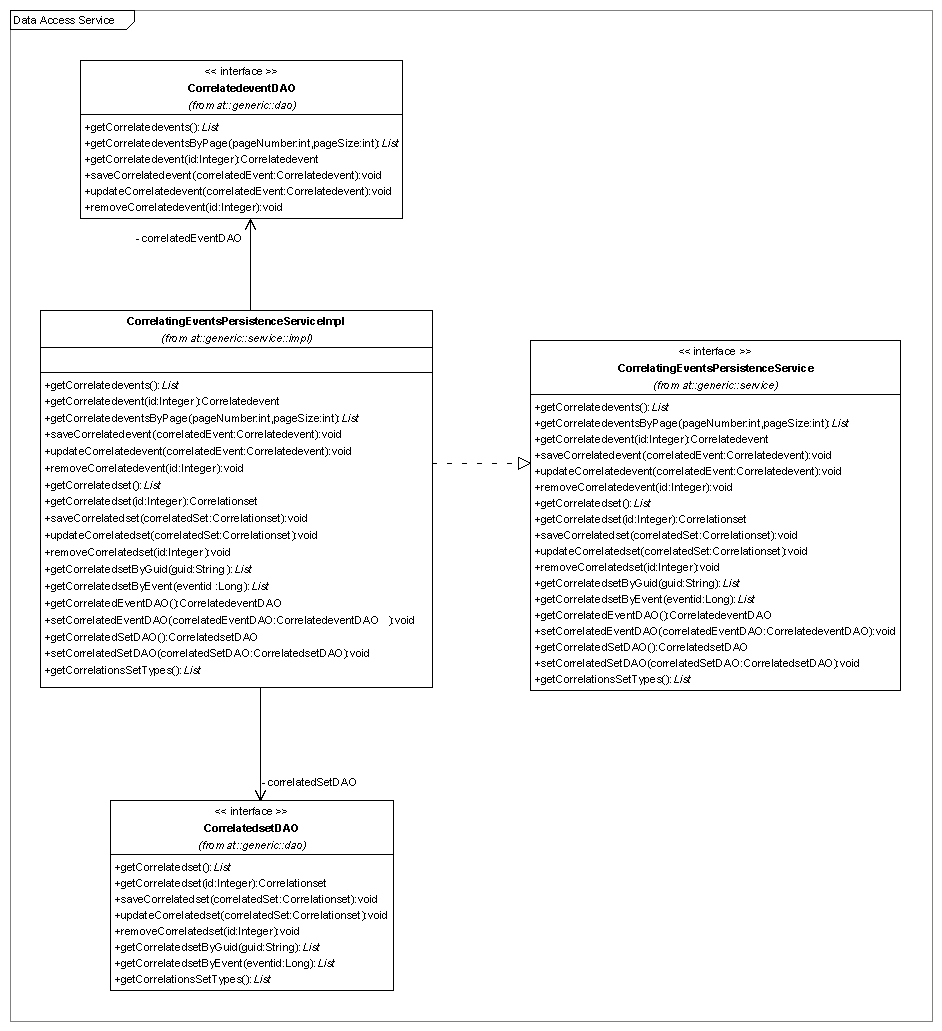
\includegraphics[width=1.0\textwidth]{pics/DataAccessServiceCorrelatedevent.png}
	\caption{CorrelatedEventsPersistenceService}             
	\label{fig:CorrelatedEventsPersistenceService}
\end{figure}            
%***************************************

%***************************************
\begin{figure}[h!]  
	\begin{mytinylisting}
	\begin{verbatim}
	<bean id="correlatingEventsPersistenceService" class="at.generic.service.impl.CorrelatingEventsPersistenceServiceImpl"> 
    	<property name="correlatedEventDAO">
    		<ref bean="correlatedEventDAOTarget"/>
    	</property> 
    	<property name="correlatedSetDAO">
    		<ref bean="correlatedSetDAOTarget"/>
    	</property> 
    </bean>
    \end{verbatim}
    \end{mytinylisting}
	\caption{EventPersistenceService}             
	\label{lst:EventPersistenceService}
\end{figure} 
%***************************************

The AdminService provides a service for misc. admin oeprations that has to be persisted including role and filter managment for example (Figure \ref{fig:AdminPersistenceService} and Listing Figure \ref{lst:EventPersistenceService}).
\\\\
%***********************
\begin{figure}[h!]                                  
	\centering                                           
	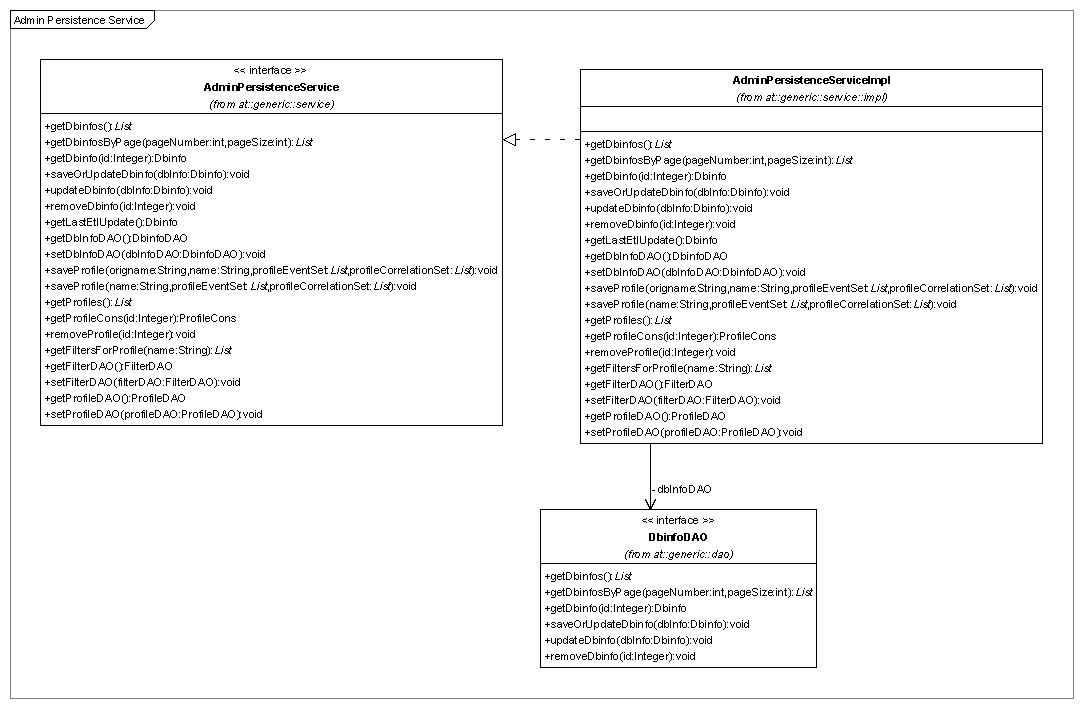
\includegraphics[width=1.0\textwidth]{pics/AdminPersistenceService.png}
	\caption{AdminPersistenceService}             
	\label{fig:AdminPersistenceService}
\end{figure}            
%***************************************

%***************************************
\begin{figure}[h!]  
	\begin{mytinylisting}
	\begin{verbatim}
	<bean id="adminPersistenceService" class="at.generic.service.impl.AdminPersistenceServiceImpl"> 
    	<property name="dbInfoDAO">
    		<ref bean="dbInfoDAOTarget"/>
    	</property> 
    </bean>
    \end{verbatim}
    \end{mytinylisting}
	\caption{EventPersistenceService}             
	\label{lst:EventPersistenceService}
\end{figure} 
%***************************************

%**************************************************************************************
\newpage
\subsection{Loading Process}
%**************************************************************************************
The Intime database provides the events with different information (Listing Figure \ref{lst:SourceEvent}). Each event comes with a unique id, a creation time and the event itself as an xml. The attributes from the OrderReceived root node are basic key-value pairs that are stored straight forward into the events relation. 
\\\\
The more tricky part is the extraction of each attribute and their validation against its definiton. The datatypes of each attribute are extracted and stored into the database as well. A lot of work in this process is done by the EventPeristenceServices as it autmatically takes care about saving eventtypes and timepoints. 
\\\\
This process is pretty forward as the user only has to provide event definitons and register the new events in Spring's context configuration. The user can controll and supervise the loading process from the web user interface in the admin section. By clicking the Button "Start Transformation" a thread is triggered that is collecting the events from it source and transforms them into the target database schema. During this process the full text index is created or update which is done by using the Indexer interface (Figure \ref{fig:etlProcess}).

% TODO: screenshot vom adminteil reingeben 

%***************************************
\begin{figure}[h!]  
	\begin{mytinylisting}
	\begin{verbatim}
	<OrderReceived 
		guid="ec3db221-3f65-48cc-9982-7bf781fab3b7" 
		originalGuid="8f2cf907-5e5f-4f0c-8aa8-e07ab521d1a9" 
		priority="Medium" severity="Unknown" 
		localTimeCreated="2006-03-04T17:31:29.6085000+01:00" 
		localTimeCreatedRW="2006-03-04T17:31:29.6085000+01:00" 
		utcTimeCreated="2006-03-04T16:31:29.6085000+01:00" 
		utcTimeCreatedRW="2006-03-04T16:31:29.6085000+01:00" 
		majorVersion="1" 
		minorVersion="0">
		
		<OrderId>1000</OrderId>
		<DateTime>2005-11-01T07:00:00.0000000+01:00</DateTime>
		<DeliveryDate>2005-11-07T15:47:00.0000000+01:00</DeliveryDate>
		<Destination>Paris</Destination>
		
		<ProductCollection>
			<Product>
				<ProductId>Arzeutic</ProductId>
				<Amount>800</Amount>
			</Product>
		</ProductCollection>
	</OrderReceived>
    \end{verbatim}
    \end{mytinylisting}
	\caption{Source Event}             
	\label{lst:SourceEvent}
\end{figure} 
%***************************************

%***********************
\begin{figure}[!h]                                  
	\centering                                           
	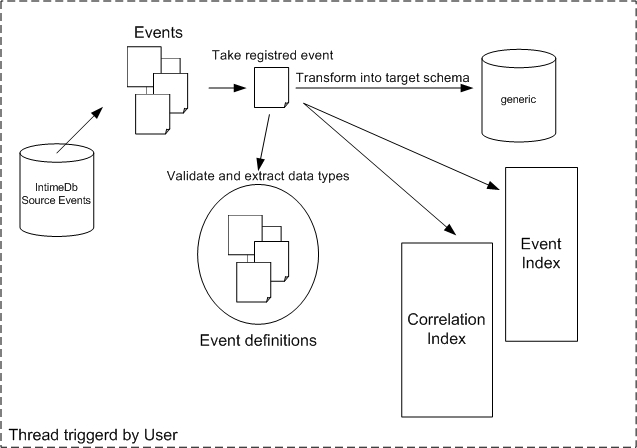
\includegraphics[width=1.0\textwidth]{pics/etlProcess.jpg}
	\caption{ETL Process}             
	\label{fig:etlProcess}
\end{figure}            
%***************************************

%**************************************************************************************
\subsection{Spring IoC container}
%**************************************************************************************
During the time when Java programming reached its critical mass of users Sun Microsystems published the Enterprise Java Beans 1.0 specifications (1998). EJB is a server side component settled in the middle layer of an enterprise application. Its major goal is to improve distribution transparency and reusability of components underlined by the statement that EJBs should make developing enterprise systems easier. EJB actually was the first technology that allowed decelrative transactions for instance. 
\\\\
As time went by the first enthusiasm had gone and experiences with EJB have shown that they don't necessarily hold what they promised. This problem has been addressed by Rod Johnson in first place (\cite{Johnson02}). EJB addresses just too many problems thus results in a high complexity. As most applications don't need the most addressed features EJBs create too much overhead. 
\\\\
Rod Johnson propagets following major flaws of EJBs based on his experience \cite{Johnson02}:
\begin{itemize}
	\item It brings too much unnecessary complexity with it.
	\item Through EJB's complexity provided the productivity is low and the probability of erros grow
	\item Automated unit testing is poorly supported
	\item Huge amounts of problem specifications have been worked in but only a slight percentage addresses common real world problems.
	\item Entity Beans have failed.
	\item EJB system have a relativly poor performance and don't scale up well.
	\item Too much code has to be produced which resulted in various code generators that make maintainability problematic.
	\item EJBs promised to be plattform independent. In reality applications became EJB container vendor specific.
\end{itemize}

The quesion arises "Why use J2EE and EJBs at all then?". The answear is that J2EE provides a wide range of usefull services and standards that can be integrated into applications without the use of EJBs. Spring's goal is to deliver those services to the user by simplifying the programmming model using only simple POJOS (\cite{SpringInAction05}).
\\\\
\textit{Spring is a lightweight inversion of control and aspect-oriented container framework.} \cite{SpringInAction05}
\\\\
Spring is acutally a lightweigt container that provides an inversion of control (IoC) which means that it is capable of managing the life cycle and configurations of its beans. The inversion of control pattern makes it possible to write the applications business logic completle unaware of its underlying technology. Spring provides means of creating dependcies without any intrusion into business code. That is a major feature which allows to develop loosly coupled and highly scalable components. The developer can concentrate only solving business problems and creating easily reusable components. It is possible to remove the complete Spring support from the application without affecting any business code written. Using the Spring Framework the developers are forced to program against interfaces and the concrete implementation of the code are wired in by configuration files using Spring. Another enriching feature is that Spring makes extensive use of the aspect oriented programing (AOP) paradigm which is used to seperate business logic from system services like transaction managment seen the previous section. The transaction managment of the data access is completely seperated from the code and even the Hibernate specific implementation parts can be changed in a minute using the configuration power of Spring. 
\\\\
The Spring Framework is composed of several main components:
\begin{itemize}
	\item Core container
	\item O/R Mapping modules
	\item Application Context Modules
	\item JDBC and DAO modules
	\item MVC Framework
\end{itemize}

The core of Spring Framwork is undisputable the core container and the the application context module. The core containers heart is the BeanFactory which lets the user wire the components together. It uses the Factory Pattern to realize dependency injections and to control the objects life cycles. The BeanFactory supports two types of objects: Singelton and Prototype. The singelton creates a shared instance of an object which is addressed by a name and mostly used as an stateless object. The prototype allows to create an independent instace for each reference of this class.
\\\\
The O/R and DAO modules have been discussed in detail in the previous sections.
\\\\
\\\\
The business logic should always be laid inside simple Java Beans with according getters and setters to its dependent objects to enable the dependency injection by the BeanFactory. These beans are implemented against a previously defined interface. For example the SearchService is an interface to a Java Bean that has got references to other beans with according getters and setters. These beans are defined in the application context and their implementations and dependecies are wired together using the Spring Framework (Listing Figure \ref{lst:wiringbeanstogether}).

%***************************************
\begin{figure}[h!]  
	\begin{mytinylisting}
	\begin{verbatim}
	<bean id="indexingServiceCorrEvents" class="at.generic.search.impl.LuceneIndexingImpl" init-method="init"> 
	    	<property name="indexLocation">
	    		<value>d:/luceneindex/correvents</value>
	    	</property> 
	</bean>    

 	<bean id="searchService" class="at.generic.search.impl.SearchServiceImpl"> 
    	<property name="indexingServiceCorrEvents">
    		<ref bean="indexingServiceCorrEvents"/>
    	</property> 
    	<property name="indexingServiceEvents">
    		<ref bean="indexingServiceEvents"/>
    	</property> 
    	 <property name="eventPersistenceService">
    		<ref bean="eventPersistenceService"/>
    	</property> 
    	<property name="corrPersistenceService">
    		<ref bean="correlatingEventsPersistenceService"/>
    	</property>
    	<property name="maxSearchResults">
    		<value>10</value>
    	</property>
    </bean>    
    \end{verbatim}
    \end{mytinylisting}
	\caption{Wiring beans together.}             
	\label{lst:wiringbeanstogether}
\end{figure} 
%***************************************
% *********************
% TODO:
% - IoC und AOP genauer beschreiben!
% ******************
%**************************************************************************************
\subsection{Spring MVC}
%**************************************************************************************
The MVC pattern was originally introduced Smalltalk developed in the 70s at the Xerox Palo Alto Research Center. Its main purpose was to manage the GUI and user interactions for the first graphic-window based applications. The MVC pattern is used to seperate the representation, processing and data components to achieve a loosly couple design which results in a clean reusable and maintainable code. 
\\\\
The three main seperations are:
\begin{itemize}
	\item \textbf{Model:} Represents the underlying domain models which are usually populated by a database like in Event Cloud the event models.
	\item \textbf{View:} This component is mainly responsible for presenting the data and the user interface. In a webbase application this is normally done using JSP/JSTL to render HTML pages containg some data.
	\item \textbf{Controller:} This is the core component which handles the coordination. It is responsible of processing user inputs, delegating requests to business processes and coordingating the representation of results.
\end{itemize}
Spring Framework brings a full blown MVC framework with it to help to develop web applications in a fast and efficient way. Spring's MVC comes with a rich set of features:

\begin{itemize}
	\item automatic population of models according to request parameters
	\item declarative validation
	\item state managment through web forms
	\item workflow coordination
\end{itemize}

Spring's MVC life cycle is presented in the Figure \ref{fig:SpringMVC}. The DispatcherServlet is receiving the a user request and queries the according mapping for the specific request. The HandlerMapping is simply mapping URLs to controllers. The Dispatcher is delegating the request to the according controller once it resolved the mapping. The Controller job is to perform some business operations in sense that it delegates the workload to business objects like the service API provided by Event Cloud. After work has been done the Controller populates so called Command Models that hold all information that is needed to be shown to the user and returns a ModelAndView object to the Dispatcher that contains command model and a view name. The ViewResolver is then responsible to resolve the viewname and map it to the according view. In Event Clouds case this is a JSP page which only performs JSTL operations with display formatting routines to generate the desired HTML rendered information to its user. 
\\\\
An important feature that Spring MVC provides is that it is possible to create interceptors for specific mappings and controllers compareable to servlet filters. This allows to implement access control for instance in no time and without to touch any controller. This provides an extremly loosly coupled design as no code is touched when implementing such a thing.   

%***********************
\begin{figure}[!h]                                  
	\centering                                           
	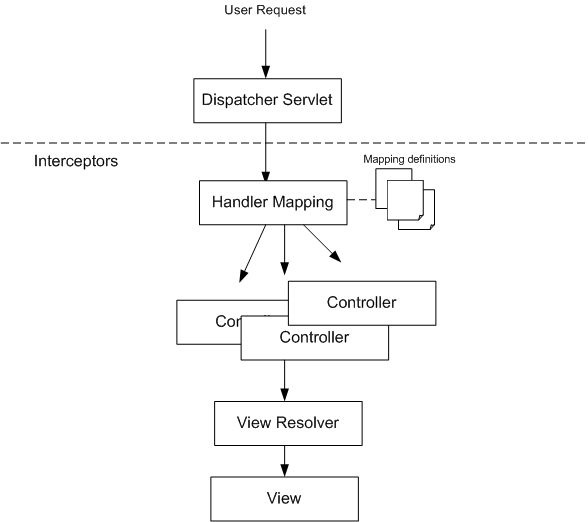
\includegraphics[width=1.0\textwidth]{pics/SpringMVC.jpg}
	\caption{Spring MVC}             
	\label{fig:SpringMVC}
\end{figure}            
%***************************************

To give a clear picture how this works in Event Cloud there is a Listing Figure \ref{lst:urlMapping} provided for understanding the principle of configuring Spring's MVC in Event Cloud. The first one shows how the controllers are mapped to a requested URLs. For matter of simplicity only the process of resolving the Event Clouds admin page is explained.  The admin's controller is bind to a specific object which takes several bean dependencies as arguments. The admin controller itself does not perform any business logic. It just determines what kind of request got in and decides which operation should be executed like the etl process or the creation of filter profile. Afterwards it creates an instance of a command object that holds the data to be displayed for example which Events have been indentified, when the last update process has been executed and stuff like that. When finished performing business operations it returns a ModelAndView object including the according view name to be resolved and the the name of the command object that is used by the jsp page to access it (Listing Figure \ref{lst:MVCByAdminController}). 
\\\\
The openSessionInViewInterceptor used in this excerpt is a workaround to provide access for lacy loading in the view component.

\begin{figure}[h!]  
\begin{mytinylisting}
\begin{verbatim}
	<!bean id="urlMapping"     
			class="org.springframework.web.servlet.handler.SimpleUrlHandlerMapping"> 
		<property name="interceptors">
	        <list>
				<!-- Interceptor f�r Lacy Loading im View -->
	             <ref bean="openSessionInViewInterceptor"/>
	        </list>
		</property>
       	<property name="mappings">
			<props>
				<prop key="/admin.html">adminController</prop>
			</props>
		</property>
	</bean>
	
	<bean name="adminController" class="at.generic.web.AdminController">
  		<property name="sourceEventEtl">
			<ref bean="sourceEventEtl"/>
		</property>
		<property name="adminPersistenceService">
			<ref bean="adminPersistenceService"/>
		</property>
		<property name="eventPersistenceService">
			<ref bean="eventPersistenceService"/>
		</property>
		<property name="indexingServiceEvents">
			<ref bean="indexingServiceEvents"/>
		</property>
		<property name="indexingServiceCorrEvents">
			<ref bean="indexingServiceCorrEvents"/>
		</property>
  	</bean>
    \end{verbatim}
    \end{mytinylisting}
	\caption{URL Mapping}             
	\label{lst:urlMapping}
\end{figure} 
%********************

%********************
\begin{figure}[h!]  
\begin{mytinylisting}
\begin{verbatim}
	return new ModelAndView("admin", "adminData", adminData);
    \end{verbatim}
    \end{mytinylisting}
	\caption{ModelAndView returned by the AdminController}             
	\label{lst:MVCByAdminController}
\end{figure} 
%********************

%**************************************************************************************
\subsection{Indexing and Searching Events}
%**************************************************************************************
%**************************************************************************************
\subsubsection{Indexing Events using Lucene }
%**************************************************************************************
%**************************************************************************************
\subsubsection{Searching for events}
%**************************************************************************************
%**************************************************************************************
\subsubsection{Profiles}
%**************************************************************************************
%**************************************************************************************
\subsubsection{Query Syntax}
%**************************************************************************************
Event Cloud is using Lucene's sophisticated query parser to provide a full featured query syntax to allow the creation of complex queries for searching and retrieving events and their correlations. 
\\\\
The formal query grammar definition \cite{LuceneQueryParserAPI}:
\begin{lstlisting} [basicstyle=\ttfamily\fontsize{8}{8}\selectfont]]
Query  ::= ( Clause )*
Clause ::= ["+", "-"] [<TERM> ":"] ( <TERM> | "(" Query ")" )
\end{lstlisting}
A clause can contain either a Term expression or another nested Query. There are two distinctions between terms. There can exist a \textit{single term} like "hello" or "test" or a term can be a \textit{phrase} like "hello world" enclosed by double quotes. It is possible to combine multiple terms with boolean operators \cite{LuceneQueryDescriptionPage}. The predefined Boolean connector configured in Event Cloud for Terms is the OR operator.
\\\\
Some basic query examples are described in the table \ref{fig:rank1LuceneQueryExamples} for getting started.
\\\\
However the QueryParser is capable of much richer functionality like Fuzzy Searches and and Proximity Searches. They don't have a big importance in querying but it can be powerful tool. For example it is possible to create a fuzzy search based on the Levenshtein distance using the tilde ~ symbol plus a proximity number. For example you can search for "\textit{java~}" and it will return documents that are similar to java like lava. You can adjust the proximity by adding a value next to the tilde symbol like java~0.8. The default proximity number is 0.5.
\\\\
Another noticeable minor future is the possibility to define the relevance of search terms in a query with the carot operator $\wedge$ and a number that specifies the importance of the word. For instance if you search for "\textit{Paris$\wedge$4 London}" it will make Paris more relevant than London. The default relevance value is 1.
\\\\
Further details on this topic can be found here \cite{LuceneQueryDescriptionPage}, here \cite{LuceneQueryParserAPI} and here \cite{LuceneInAction05}.

\begin{table}[!hp]
	\begin{tabular}{|p{4cm}|p{8cm}|}
		\hline \textbf{Example} & \textbf{Description} \\
		\hline \textit{Paris} & Query will return events containing "Paris" in an Attribute. \\
		\hline  \textit{Paris London} & Query will return events containing either "Paris" or "London" in an Attribute. \\
		\hline  \textit{Paris OR London} & Query will return events containing either "Paris" or "London" in an Attribute. \\
		\hline  \textit{Paris AND London} & Query will return events containing "Paris" and "London" in an Attribute.\\
		\hline  \textit{(Paris OR London) AND Szabolcs} & Query will return events containing "Paris" or "London" but they must contain "Szabolcs".\\
		\hline  \textit{+Paris +London} & Query will return events containing "Paris" and "London" in an Attribute.\\
		\hline  \textit{+Paris -London} & Query will return events that must contain "Paris" and it is not allowed that this event contains "London" in an Attribute.\\
		\hline  \textit{+Paris NOT London} & Query will return events that must contain "Paris" and it is not allowed that this event contains "London" in an Attribute.\\
		\hline  \textit{Par*} & Query will return events containing words that start with "Par" - for instance Paris.\\
		\hline 
	\end{tabular}
	\caption{Query Examples}
	\label{tab:LuceneQueryExamples}
\end{table} 

% Verwendete Patterns beschreiben
%	Facade Pattern
% 	Inversion of Control
%	Code injection

% verwendete Technologien beschreiben:
% Tomcat
% Hibernate als OR Mapping
% Datenbank Postgres
% Spring
% MVC Konzept
% Spring MVC
% Lucene



% ETL Prozess
% 	Hibernate als OR Mapping
%		Wie schauen definition files aus
%	Datenbank Postgres

% Indexing 
%	Lucene index structur
%	Verwendung von Lucene als Codebeispiel
%	Caching Themen
%	Darauf eingehen wie man

% Suche
% 	web interface 
%	Spring framework
%	Spring MVC - MVC Konzept im allgemeinen

% Beschreibung der API
%	UML Bilder und beschreiben was was macht


%**************************************************************************************
%\newpage
%\subsubsection{Evolution}
%**************************************************************************************

%**************************************************************************************
%\newpage
%\subsection{Performance}
%**************************************************************************************

%**************************************************************************************
%\newpage
%\subsection{Simulation}
%**************************************************************************************

%**************************************************************************************
\section{Appendix}
%**************************************************************************************
%**************************************************************************************
\newpage
\begin{landscape}
\section{Data Access Diagram}
%**************************************************************************************
%***********************
\begin{figure}[!h]                                  
	\centering                                           
	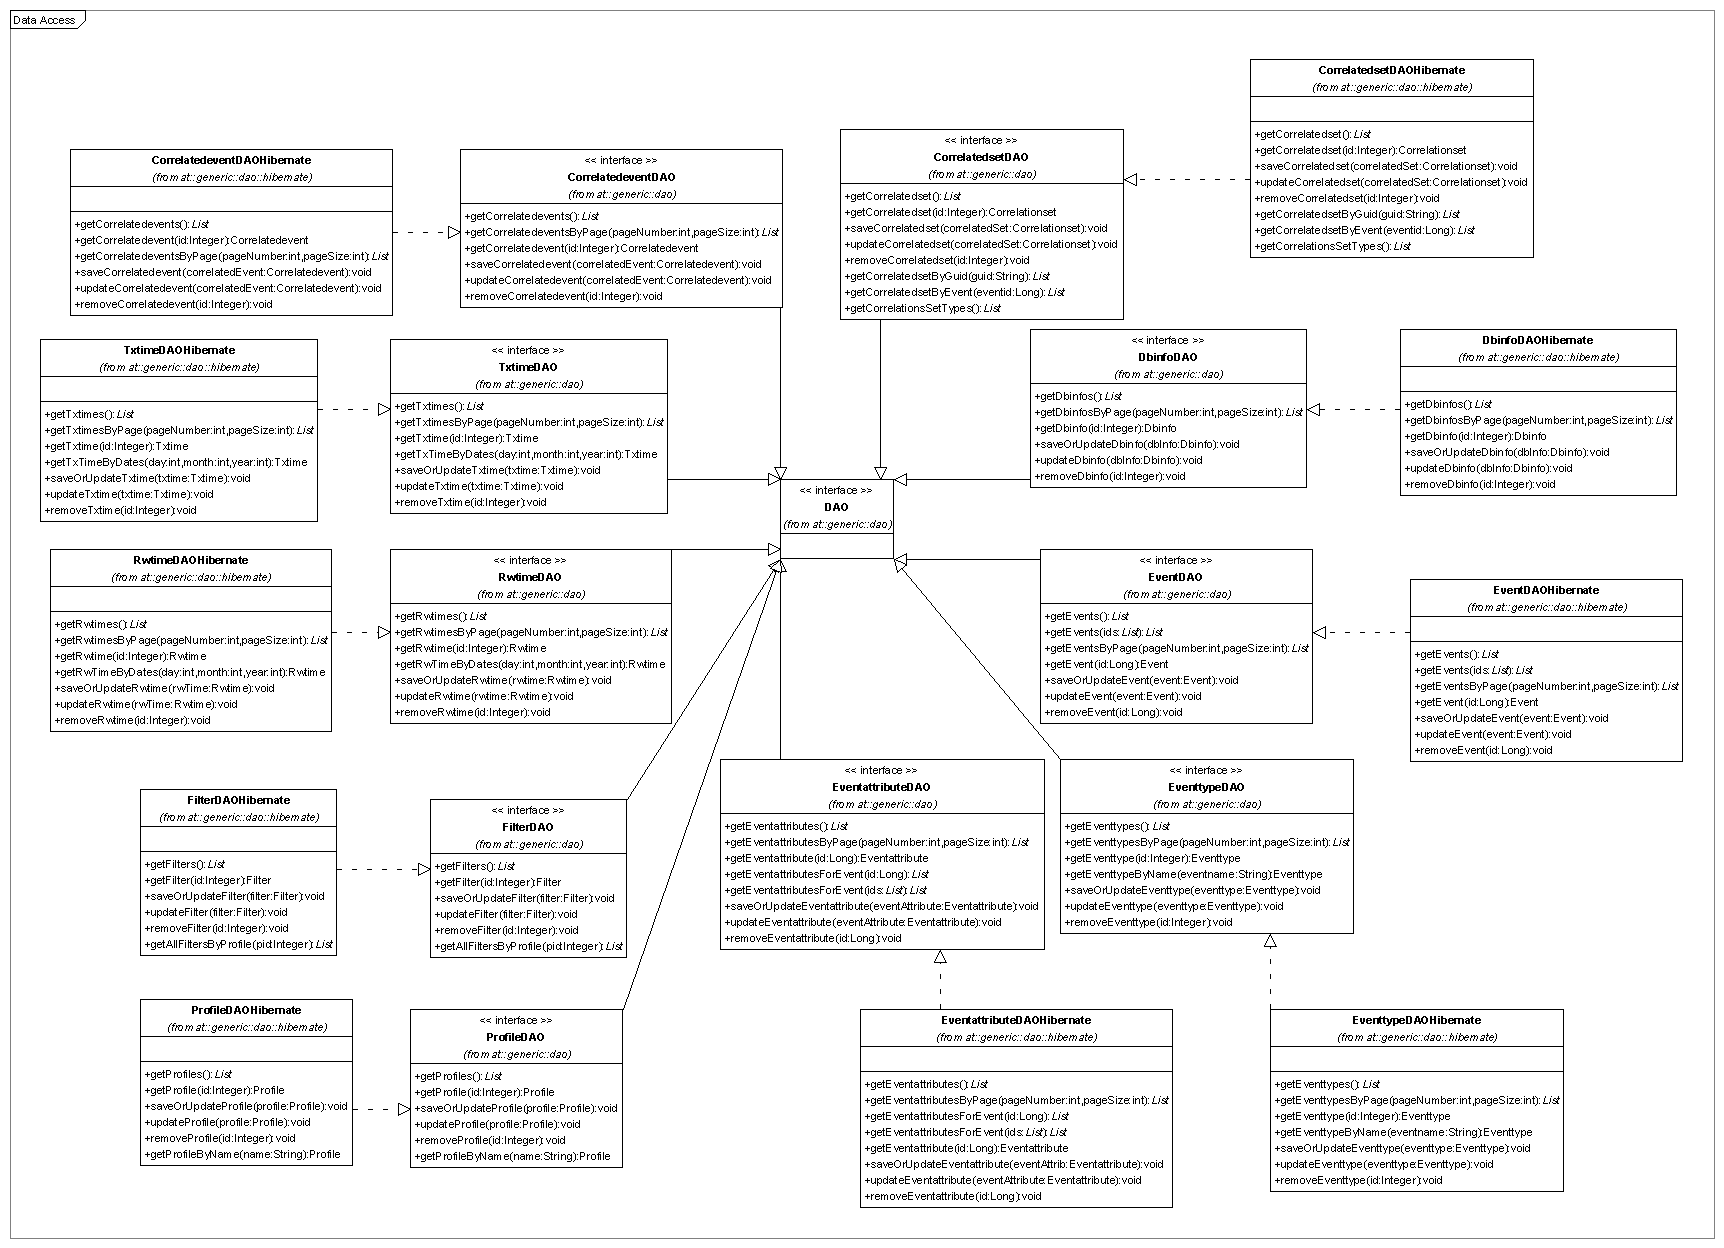
\includegraphics[width=1.1\textwidth]{pics/DataAccess.png}
	\caption{Data Access}             
	\label{fig:GeneralDataAccess}
\end{figure}            
%*********************** 
\end{landscape}
\newpage
%\lstlistoflistings
\bibliographystyle{alpha}
\bibliography{eventcloud}

\end{document}
